\chapter{M\lowercase{ultiple} D\lowercase{ynamics} M\lowercase{odels}} 

\section{Introduction}
We now begin to address the question of how to incorporate useful prior knowledge regarding the dynamics of a system into the probabilistic learning framework. In this chapter we deal with the problem of how to include known, or approximate, relationships between state variables. An important example of such a relationship is state variables that are related as time derivatives. In other words, position-velocity relationships. Another example would be higher order Markov systems where the system ``state" actually depends on a number of delayed ``states". Further, the task of tracking a known reference signal, or distribution of reference signals, could be contrived as a known relationship between state variables. With the probabilistic learning framework we have derived thus far, it is not clear how such information could be incorporated. We provide a novel method that tackles this problem.

%Often prior knowledge will come in the form of known, or approximate, relationships between a subset of the system state variables. In other words, the state-space may be partitioned into states with known dynamics and states with initially unknown dynamics. An obvious example of this is position-velocity relationships. However, more general problems may be tackled. The task of tracking a reference signal with a given linear combination of states in which the control policy may have access to some preview horizon of the reference can also be tackled by this framework. A further example is higher order Markov systems where the system ``state" actually depends on a number of delayed states.

Once we have formulated a method to achieve the goal of incorporating known state relationships we would like to investigate what effect their inclusion will have on learning. In particular we would like to investigate whether learning can proceed faster, both computationally and in terms of finding a good policy, and what is the propensity for finding good (or bad) local minima in completing the task.

Our method is formulated by considering that the system we are dealing with can be decomposed as multiple dynamics models all acting on different parts, or linear transformations, of the state-action vector. We shall use the terms \textit{multiple dynamics} and \textit{augmented dynamics} interchangeably when referring to this framework. In order to fit into the probabilistic framework, the use of multiple dynamics must satisfy the propagation of uncertainty criteria outlined in the previous chapter. It is this problem that we tackle now.


\section{Augmented Dynamics} \label{sec:augmentedDYN}
\subsection{Framework}

Consider the case in which the system dynamics function $\bff$ consists of the concatenation of $M$ distinct functions
\begin{equation}
\bff(\bz) = \bff_{1:M}(\bz) := \bmat{\bff_1(\bz) \\ \vdots \\ \bff_M(\bz)}
\label{eqn:multimodel}
\end{equation}
Each sub-function (or sub-dynamics) $\bff_m$ can explicitly depend on any of the previous functional outputs $\bff_{1:m-1}$ as well as the state-action $\bz$. In mathematical terms $\bff_m(\bz) = \bff_m\big(\bz,\bff_{1:m-1}(\bz)\big)$ for $m \in \ZZ_{[2,M]}$. We define the concatenation of the state-action and the $m-1$ previous functions as
\begin{equation*}
\bp_m(\bz) = \bmat{\bz \\ \bff_{1:m-1}(\bz) }
\end{equation*}
where $\bp_1(\bz) = \bz$ as this will be helpful later on. To see how this setup is beneficial for encoding position-velocity relationships or incorporating reference signals we show how they can be phrased in this framework using the following examples.

\begin{exa}[Position-Velocity] Consider a system with time derivative related states $\bx = [\ba; \dot\ba]$ where the positions $\ba$ evolve according to the dynamics $\ba_+ = \bff_1(\bz)$. The velocities $\dot\ba$ could then be reconstructed using some approximate relationship $\dot\ba_+ = \bff_2\big(\bz,\bff_1(\bz)\big)$, for example a linear relationship $\dot\ba_+ = \bM\big[\bz;\bff_1(\bz)\big]$. One setting for such a matrix could be $\bM = [-\bI, \bO, \bI]/\Dt$ which would encode the relationship $\dot\ba_+ = (\ba_+ - \ba)/\Dt$ which is reasonable for small $\Dt$. This example will be pursued further in \Sec{posvel}.
\end{exa}

\begin{exa}[Reference Generator] Consider a system with dynamics $\bx_+ = \bff_1(\bz)$ which has been tasked to track a some reference signal $\br$. Now assume that this reference comes from some underlying dynamical system $\bx^\br_+ = \bff_2(\bx^\br)$ where $\br = \bC^\br\bx^\br$. The dynamics of the system itself $\bx$ can then be augmented with the state of the reference system $\bx^\br$ such that the reference state simply becomes part of an augmented state space. Note that the function $\bff^\br$ could be provided by the user or inferred from data along with the system dynamics. How this setup can be used for learning reference tracking will be explored in \Sec{reffy}.
\end{exa}


In order to fit into the probabilistic framework of the previous chapter it is necessary for us to build up a moment-matched Gaussian approximation $\bff(\bz) \sim \cN(\bm_*, \bS_*)$ given $\bz \sim \cN(\bm,\bS)$. \Ass{gauss} states that $\bm_* = \EE_{\bz,\bff}[\bff(\bz)]$ and $\bS_* = \cov_{\bz,\bff}[\bff(\bz)]$. However, further approximations will have to be made in the case of multiple dynamics models since these moments cannot be calculated for general sub-functions even if the moments of each can be evaluated individually. 


\begin{ass} \label{ass:multigauss}
Given $p(\bz)$ is Gaussian, the resulting distribution of the next state $p\big(\bff(\bz)\big)$ is replaced by the Gaussian distribution
\begin{equation*}
\bff(\bz) \sim \cN\left(
\bmat{\EE_{\bz,\bff_1}[\bff_1(\bz)] \\ \vdots \\ \EE_{\brho_M,\bff_M}[\bff_M(\brho_M)]},
\bmat{\cov_{\bz,\bff_1}[\bff_1(\bz)] & \dots & \cov_{\brho_M,\bff_M}[\bff_1(\bz),\bff_M(\brho_M)] \\
\vdots & \ddots & \vdots \\
\cov_{\brho_M,\bff_M}[\bff_M(\brho_M),\bff_1(\bz)] & \dots & \cov_{\brho_M,\bff_M}[\bff_M(\brho_M)]}
\right)
\end{equation*}
where $p(\brho_m)$ is the moment matched approximation of the real distribution $p\big(\bp_m(\bz)\big)$.
\end{ass}

Note that this is an iterative extension of \Ass{gauss}. As before, we shall no longer make a distinction between the real distribution $p\big(\bp_m(\bz)\big)$ and its approximation $p(\brho_m)$.
%
Propagation of uncertainty is now reduced to the iterative procedure of evaluating the mean $\EE_{\bp_m,\bff_m}\big[\bff_m\big(\bp_m(\bz)\big)\big]$ and covariance $\cov_{\bp_m,\bff_m}\big[\bff_m\big(\bp_m(\bz)\big)\big]$ for each dynamics model, given the assumed joint Gaussian over the previous values $\bp_m(\bz) \sim \cN$. This is possible provided that these moments can be evaluated for each sub-dynamics.

Now in order to fill out the full covariance matrix, given \Ass{multigauss}, the cross terms $\cov_{\bp_m,\bff_m}\big[\bff_m\big(\bp_m(\bz)\big), \bp_m(\bz)\big]$ are required. It turns out that if the mean $\EE_{\bp_m,\bff_m}[\bff_m\big(\bp_m(\bz)\big)]$ is differentiable with respect to the input mean $\bm = \EE_{\bp_m}[\bp_m(\bz)]$ then this term can always be evaluated as
%
\begin{align}
\cov_{\bp_m,\bff_m}\big[\bff_m\big(\bp_m(\bz)\big), \bp_m(\bz)\big] &= \bigg(\diff{}{ \bm } \EE_{\bp_m,\bff_m}\big[\bff_m\big(\bp_m(\bz)\big)\big] \bigg) \bS
\label{eqn:multicov}
\end{align}
%
where $\bS = \cov_{\bp_m}[\bp_m(\bz)]$ is the input covariance. This expression holds due to \Theo{inpout}. This theorem lies at the heart of the multi-model framework. While it is a straightforward derivation, this result was unknown to us from the literature, therefore the derivation is our own.


\begin{theo}[Output-Input Covariance] \label{theo:inpout}
Consider two random vectors $\ba$ and $\bb$ where $\bb$ is functionally dependent on $\ba \sim \cN(\bm,\bS)$. Then the following statement is true
\begin{equation*}
\diff{}{ \bm }\EE_{\ba,\bb}[\bb] =  \cov_{\ba,\bb}[\bb,\ba] \bS^{-1}
\end{equation*}
\espa
\end{theo}



\begin{proof}
The proof follows directly from the definition of expectation and covariance
\begin{align*}
\diff{}{\bm}\EE_{\ba,\bb}[\bb]
&= \int \EE_{\bb}[\bb] \bigg( \diff{}{\bm} \cN\big(\ba|\bm,\bS\big) \bigg) \dd\ba  \\
&= \int \EE_{\bb}[\bb] \Big(  (\ba - \bm)\T \bS^{-1} \cN\big(\ba|\bm,\bS\big) \Big) \dd\ba
\end{align*}
Now expanding out the brackets yields the expression
\begin{flalign*}
\qquad\qquad\qquad\qquad\quad\;\;
\diff{}{\bm}\EE_{\ba,\bb}[\bb]
&= \bigg( \EE_{\ba,\bb}[\bb \ba\T] - \EE_{\ba,\bb}[\bb] \bm\T \bigg) \bS^{-1}   \\ &
= \cov_{\ba,\bb}[\bb,\ba] \bS^{-1} & \blacksquare
\end{flalign*}
\end{proof}

Note that the assumption of joint Gaussianity is equivalent to assuming linear relationships between dynamics models. To see this, observe that \Eq{multicov} is in the form of a Jacobian matrix (or linearised dynamics) multiplied by the input covariance.





\subsection{Subset of Inputs}
Often the case will be that each dynamics model is only functionally dependent on a subset, or linear transformation, $\bs_m(\bz)$ of the state-actions and outputs of previous functions $\bp_m(\bz)$. How then is the expectation and covariance with respect to $\bp_m(\bz)$ to be filled in? The answer can be found by considering the general linear transformation $\bs_m(\bz) = \bP_m\bp_m(\bz)$. The matrix $\bP_m$ could either pick off appropriate elements of $\bp_m$ or be viewed as an arbitrary linear combination. Since this mapping is linear, a Gaussian distribution $\bp_m(\bz) \sim \cN(\bm,\bS)$ leads to another Gaussian distribution $\bs_m(\bz) \sim \cN\big(\bm_{\bs},\bS_{\bs}\big)$ with mean $\bm_{\bs} = \bP_m\bm$ and covariance $\bS_{\bs} = \bP_m\bS\bP_m\T$. Therefore the predictive mean and covariance are simply
\begin{align*}
\EE_{\bp_m,\bff_m}\big[\bff_m\big(\bp_m(\bz)\big)\big] &= \EE_{\bs_m,\bff_m}\big[\bff_m(\bs_m(\bz)\big)\big] \\
\cov_{\bp_m,\bff_m}\big[\bff_m\big(\bp_m(\bz)\big)\big] &= \cov_{\bs_m,\bff_m}\big[\bff_m\big(\bs_m(\bz)\big)\big]
\end{align*}
In order to obtain the cross covariance term $\cov_{\bp_m,\bff_m}\big[\bff_m\big(\bp_m(\bz)\big), \bp_m(\bz)\big] = \cov_{\ba,\bb}[\bb,\ba]$ first define $\bc = \bs_m(\bz)$. Then note that, since $\bb$ is only affected by $\ba$ through $\bc$, the conditional independence relationship $\ba \ci \bb | \bc$ holds. This relationship can be represented by the graphical model shown in \Fig{condind}. Due to the joint Gaussian assumption, \Theo{condind} can be appealed to. This theorem is well known in the Machine Learning community.






%-------------------------------------------------------------------------------------------------------------------------------------------
\begin{figure}[t]
\centering
%
\tikzstyle{sum} = [circle, draw, minimum height=.8cm]
\tikzstyle{line} = [draw, -latex]
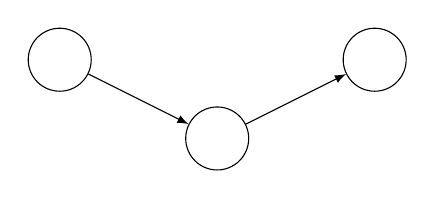
\begin{tikzpicture}
	\node[sum] (a) at (-2,0) {$\ba$}; 
	\node[sum] (b) at (0,-1) {$\bc$};
	\node[sum] (c) at (2,0) {$\bb$};
	\path[line] (a) -- (b); \path[line] (b) -- (c);
\end{tikzpicture}
%
\caption{Graphical model for which the conditional independence relationship $\ba \ci \bb \big| \bc$ holds. See \cite{Bish06} Chapter 8.2 for a more detailed outline.}
\label{fig:condind}
\end{figure}
%-------------------------------------------------------------------------------------------------------------------------------------------





\begin{theo}[Conditional Independence] \label{theo:condind}
Take three random vectors $\ba,\bb$ and $\bc$ which are jointly Gaussian distributed. Given $\ba \ci \bb | \bc$ the following statement is true
\begin{equation*}
\cov[\bb,\ba] = \cov[\bb,\bc] \cov[\bc]^{-1} \cov[\bc,\ba]
\end{equation*}
\end{theo}

\begin{proof}
Consider the joint distribution $p(\ba,\bb,\bc)$ partitioned as follows
\begin{equation*}
\bmat{\ba \\ \bb \\ \bc} \sim \cN \left(
\bmat{\bm_{\ba} \\ \bm_{\bb} \\ \bm_{\bc}},
\bmat{
\bS_{\ba} & \bS_{\ba\bb} & \bS_{\ba\bc} \\
\bS_{\bb\ba} & \bS_{\bb} & \bS_{\bb\bc} \\
\bS_{\bc\ba} & \bS_{\bc\bb} & \bS_{\bc}
} \right)
\end{equation*}
Conditioning $\ba$ and $\bb$ on $\bc$ using the identity for a Gaussian conditional distribution yields the cross covariance term
\begin{equation*}
\cov[\bb,\ba|\bc] = \bS_{\bb\ba} - \bS_{\bb\bc} \bS_{\bc}^{-1} \bS_{\bc\ba}
\end{equation*}
This expression is equal to zero since the conditional independence relationship $\ba \ci \bb | \bc$ can be stated equivalently as $\cov[\ba,\bb|\bc] = \bO$. The result follows from a rearrangement of terms.
\qed
\end{proof}

However, computing the inverse of the potentially singular matrix $\cov[\bc]$ is unsatisfactory. Fortunately, explicit calculation of this inversion is unnecessary since $\cov[\bb,\bc] \bS_{\bs}^{-1} = \dd\EE[\bb]/\dd\bm_{\bs}$ due to \Theo{inpout}. Therefore the cross covariances can be expressed as
\begin{align*}
\cov_{\bp_m,\bff_m}\big[\bff_m\big(\bp_m(\bz)\big), \bp_m(\bz)\big]
&= \bigg(\diff{}{ \bm_{\bs} } \EE_{\bs_m,\bff_m}[\bff_m\big(\bs_m(\bz)\big)\big] \bigg) \bP_m \bS
\end{align*}
where $\bP_m\bS = \cov[\bc,\ba]$. The full framework for propagating uncertainty using multiple dynamics models was implemented in MATLAB and can be found in \App{codeCost} implemented by the function \texttt{propagated.m}. This function has been developed by multiple contributors where the author's main contributions to it were the multiple dynamics framework and the derivative calculations using the vectorisation convention of \App{matcal}.

This concludes the definition of the framework for propagation of Gaussian uncertainty given multiple dynamics models with the form in \Eq{multimodel}. Note that the only condition on each dynamics model is that the mean $\EE_{\bs_m,\bff_m}\big[\bff_m\big(\bs_m(\bz)\big)\big]$ and covariance $\cov_{\bs_m,\bff_m}\big[\bff_m\big(\bs_m(\bz)\big)\big]$ are analytically tractable for $\bs_m \sim \cN$, $\bff_m \sim \mathcal{GP}$ and that the mean is differentiable with respect to the mean of the input distribution $\bm_{\bs}$. Now some specific applications are discussed.


\subsection{Higher Order Markov Systems} \label{sec:nonmarkov}
One use of this framework that is immediately transparent is the case in which the system in question has a Markov order greater than one in its relationship to previous states. In other words, with multiple dynamics models, Markov system of order $N$ and of the form
\begin{equation*}
\bx_{k+1} = \bff\big(\bx_{k},\bx_{k-1}\dots,\bx_{k-N+1},\bu_{k}\big)
\end{equation*}
can be considered by defining the augmented state-space system
\begin{equation*}
\bx^{\aug}_{k+1} = \bmat{ \bff\big(\bx^{\aug}_{k},\bu_{k}\big) \\[0.1cm] 
\bmat{\bI & \bO} \bx^{\aug}_{k}
}
\end{equation*}
with augmented state vector $\bx^{\aug}_k = [\bx_{k}; \bx_{k-1} \dots  \bx_{k-N+1}] \in \RR^{NE}$. Obviously a similar procedure could be applied if the system also depends on delayed actions. This is a useful property that we will exploit in the subsequent sections.







\section{Known State Relationships}

\subsection{General Mappings}
The framework of multiple dynamics models outlined in the previous section finds one of its most useful applications in the incorporation of known relationships between states, a form of partial model information. This application is presented in \cite{HRM12}. Specifically, given a system composed of $M$ distinct functions as given in \Eq{multimodel}, then often some of the sub-dynamics may be fixed or known beforehand. In this case, the unknown dynamics can be inferred from data using a parametric or nonparametric method outlined in \Sec{bayesmodelling} while the known parts can be included directly. A very clear and useful example of this for dynamical systems is the case where some states are known to be time derivatives of other states. In other words, position-velocity relationships.









\subsection{Position-Velocity}
\label{sec:posvel}




Consider the common scenario in which the state $\bx$ contains \textit{position} states $\bxp$ and \textit{velocity} states $\bxv$ which are related through
\begin{align}
\bxp_k &= \int_{-\infty}^t \!\!\!\!\bxv(\tau) \dd\tau \quad\text{or}\quad
\bxp_k = \bxp_{k-1} + \int_{t-\Dt}^t \!\!\!\!\bxv(\tau) \dd\tau \label{eqn:posint} \\[0.2cm]
\bxv_k &= \frac{\dd\bxp(\tau)}{\dd \tau} \bigg|_{\tau = t} \label{eqn:veldiff}
\end{align}
where $k \in \ZZ$ and $t = k\Dt$. In order to incorporate this information into the learning framework it is important to first determine whether a predictive model for the position states is to be inferred and the velocity states reconstructed from this prediction (numerical differentiation) or vice versa (numerical integration). Approximate solutions for both cases will be discussed.



%-------------------------------------------------------------------------------------------------------------------------------------------
\begin{figure}
\centering
%
\subfigure[Integral approximations.]{
\begin{tikzpicture}
	\small
	\node at (0,0) {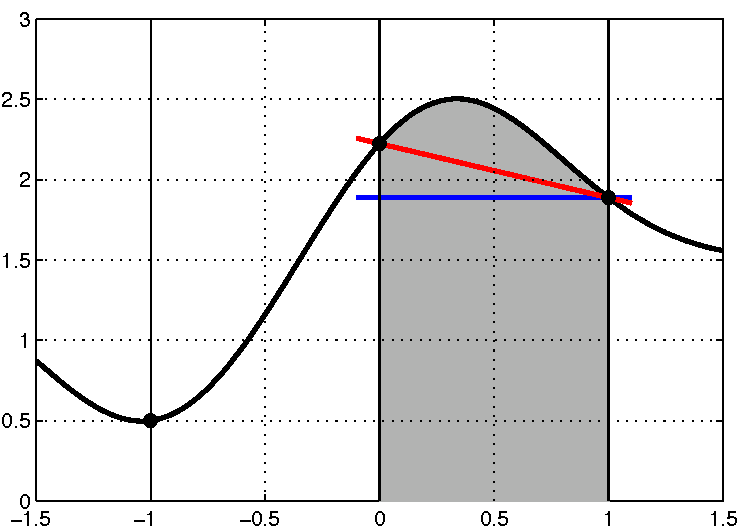
\includegraphics[scale=0.6, clip, trim=0.5cm 0.4cm 0cm 0cm]{figs/prioraug/vp1.pdf}};
	\node at (2.3,-2.8) {$t$}; \node at (3.0,-2.79) {time};
	\node at (0,-2.8) {$t-\Dt$};
	\node at (-2.3,-2.8) {$t-2\Dt$};
	\node[rotate=90] at (-3.05,1.3) {velocity $\bxv$};
	\node at (1.15,-1) {$\int_{t-\Dt}^t \bxv \dd\tau$};
\end{tikzpicture}
\label{fig:posint}
}
\hfill
\subfigure[Derivative approximations.]{
\begin{tikzpicture}
	\small
	\node at (0,0) {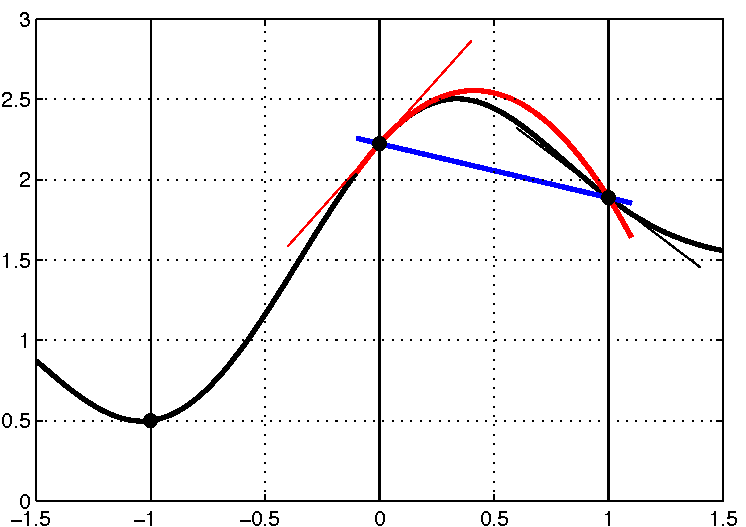
\includegraphics[scale=0.6, clip, trim=0.5cm 0.4cm 0cm 0cm]{figs/prioraug/vp2.pdf}};
	\node at (2.3,-2.8) {$t$}; \node at (3.0,-2.79) {time};
	\node at (0,-2.8) {$t-\Dt$};
	\node at (-2.3,-2.8) {$t-2\Dt$};
	\node[rotate=90] at (-3.05,1.3) {position $\bxp$};
	\node at (2.85,-0.4) {$\frac{\dd\bxp}{\dd \tau}(t)$};
\end{tikzpicture}
\label{fig:veldiff}
}
%
\caption{Approximate reconstruction of the current position/velocity states given previous observations of the velocity/position states up to time $t-\Dt$. The thick blue and red lines in each plot make approximations of zero and constant acceleration $\dot\bx^{\text{v}}$ respectively. The thin red line in plot (b) shows actual gradient at time $t-\Dt$, which the constant acceleration approximation utilises.}
\end{figure}
%-------------------------------------------------------------------------------------------------------------------------------------------


First consider the reconstruction of the position states $\bxp_k$ given the previous position $\bxp_{k-1}$ and the set of inferred velocities $\bxv_k$ and $\bxv_{k-1}$ from the probabilistic model. This corresponds to approximating the integral in \Eq{posint} which is depicted graphically in \Fig{posint}. Assuming the velocity follows a constant or linear variation (equivalently the acceleration is zero or constant across the interval) corresponds to the following approximations
\begin{align}
\bxp_k &\approx \bxp_{k-1} + \Dt\bxv_k \label{eqn:int1} \\
\bxp_k &\approx \bxp_{k-1} + \tfrac{1}{2} \Dt \Big( \bxv_k + \bxv_{k-1} \Big) \label{eqn:int2}
\end{align}
respectively. These are roughly equivalent to the Euler and Heun methods for numerical integration. Now consider reconstruction of the velocity states $\bxv_k$ given the inferred positions $\bxp_k$ and $\bxp_{k-1}$. In this case assuming the position follows a linear or quadratic variation (equivalently the acceleration is zero or constant across the interval) leads to
\begin{align}
\bxv_k &\approx \Dt\inv \Big( \bxp_k - \bxp_{k-1} \Big) \label{eqn:diff1} \\
\bxv_k &\approx 2 \Dt\inv \Big( \bxp_k - \bxp_{k-1} \Big) - \bxv_{k-1} \label{eqn:diff2}
\end{align}
respectively. This process is depicted in \Fig{veldiff}. As expected, these relationships are simply rearrangements of \Eqs{int1}{int2}. All these approximate relationships are linear and can therefore be easily incorporated into the multiple dynamics framework.






%-------------------------------------------------------------------------------------------------------------------------------------------
\begin{figure}[t]
\centering
%
\subfigure[Integral approximations.]{
\tikzstyle{line} = [draw, -stealth']
\begin{tikzpicture}
	\small
	\node at (0,0) {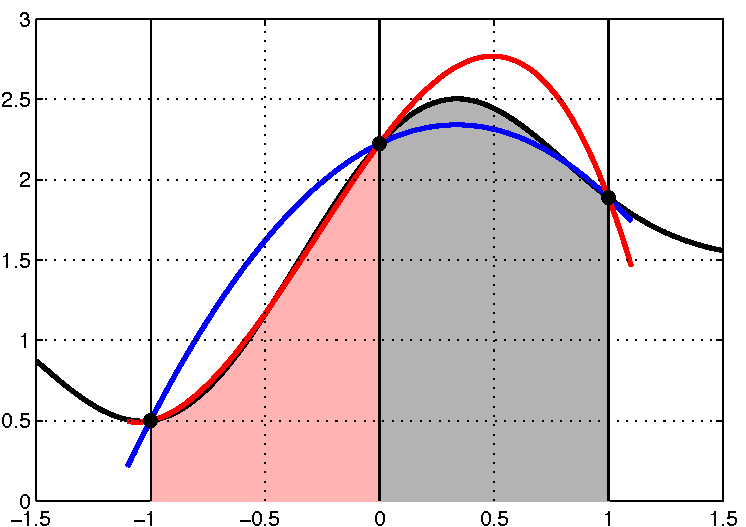
\includegraphics[scale=0.6, clip, trim=0.5cm 0.4cm 0cm 0cm]{figs/prioraug/vp3.pdf}};
	\node at (2.3,-2.8) {$t$}; \node at (3.0,-2.79) {time};
	\node at (0,-2.8) {$t-\Dt$};
	\node at (-2.3,-2.8) {$t-2\Dt$};
	\node[rotate=90] at (-3.05,1.3) {velocity $\bxv$};
	\node at (1.15,-1) {$\int_{t-\Dt}^t \bxv \dd\tau$};
\end{tikzpicture}
\label{fig:posint2}
}
%
\subfigure[Derivative approximations.]{
\tikzstyle{line} = [draw, -stealth']
\begin{tikzpicture}
	\small
	\node at (0,0) {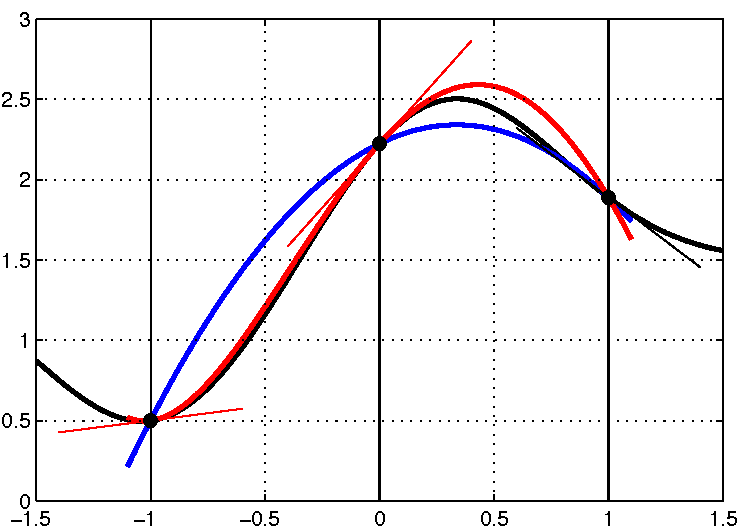
\includegraphics[scale=0.6, clip, trim=0.5cm 0.4cm 0cm 0cm]{figs/prioraug/vp4.pdf}};
	\node at (2.3,-2.8) {$t$}; \node at (3.0,-2.79) {time};
	\node at (0,-2.8) {$t-\Dt$};
	\node at (-2.3,-2.8) {$t-2\Dt$};
	\node[rotate=90] at (-3.05,1.3) {position $\bxp$};
	\node at (2.85,-0.4) {$\frac{\dd\bxp}{\dd \tau}(t)$};
\end{tikzpicture}
\label{fig:veldiff2}
}
%
\caption{Approximate reconstruction of the current position/velocity states given previous observations of the velocity/position states up to time $t-2\Dt$. The blue lines in plot (a) and (b) use only the three observed points on the graph to make a quadratic approximation of the actual curve. The red line in plot (a) additionally uses the red shaded area $\int \bxv \dd\tau$ over $[t-2\Dt,t-\Dt]$ to form a cubic approximation. This is equivalent to the red line in plot (b) which uses the derivatives $\frac{\dd\bxp}{\dd \tau}(t-\Dt)$ and $\frac{\dd\bxp}{\dd \tau} (t-2\Dt)$ shown by thin red lines to make a quartic approximation.}
\label{fig:posvel2}
\end{figure}
%-------------------------------------------------------------------------------------------------------------------------------------------





As discussed in \Sec{nonmarkov} it is not a problem to form dependencies on delayed states $\bx_{k-i}$ for $i >1$. Therefore, more elaborate approximations can be made by using information from previous timesteps. For example, fitting a quadratic curve to the points $\bxv_k, \bxv_{k-1}, \bxv_{k-2}$ or fitting a cubic curve to these points and given the area defined by $\bxp_{k-1} - \bxp_{k-2}$ yields the following approximations
\begin{align}
\bxp_{k} &\approx \bxp_{k-1} + \tfrac{1}{12}\Dt\Big( 5\bxv_k + 8\bxv_{k-1} - \bxv_{k-2} \Big) \label{eqn:dada} \\
\bxp_{k} &\approx \bxp_{k-2} + \tfrac{1}{3}\Dt\Big( \bxv_k + 4\bxv_{k-1} + \bxv_{k-2} \Big) \label{eqn:mama}
\end{align}
for position reconstruction. These approximations are shown in \Fig{posint2} by the blue and red curves respectively. Note that since there are four constraints that must be satisfied then a cubic function can do this uniquely since it has four degrees of freedom. Lower order polynomials could also be considered which would yield a unique analytic solution but would not guarantee satisfaction of the constraints.

Now, in terms of velocity reconstruction, a quadratic fit to the points $\bxp_k, \bxp_{k-1}, \bxp_{k-2}$ and a quartic fit to these points plus the derivatives defined by $\bxv_{k-1}$ and $\bxv_{k-2}$ give the relationships
\begin{align}
\bxv_{k} &\approx \tfrac{1}{2} \Dt\inv \Big( 3\bxp_{k} - 4\bxp_{k-1} + \bxp_{k-2} \Big) \label{eqn:dada2} \\
\bxv_{k} &\approx 3\Dt\inv \Big( \bxp_k - \bxp_{k-2} \Big) - \Big( 4\bxv_{k-1} + \bxv_{k-2} \Big) \label{eqn:mama2}
\end{align}
Note that the cubic fit to the velocity profile in \Eq{mama} is equivalent to the quartic fit to the position profile in \Eq{mama2}. These approximations are shown in \Fig{veldiff2} by the blue and red curves respectively.

It is important to note that using additional information from previous timesteps and higher order polynomials will not necessarily give better approximations of the integral or derivative. This is clearly shown in \Fig{posvel2} where we see that the higher order polynomial fit (thick red lines) produces a worse approximation of the required integral and derivative than the lower order fit (thick blue lines). We shall see in the following experiments whether this issue occurs in practice.


\subsection{Example: Pendulum} \label{sec:pendulum}

%-------------------------------------------------------------------------------------------------------------------------------------------
\begin{figure}
\centering
\small
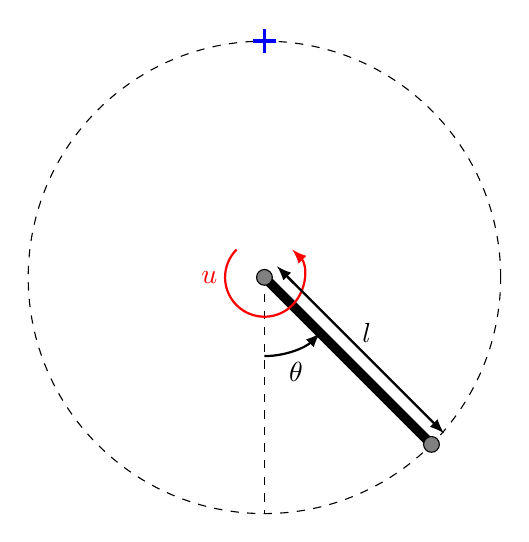
\begin{tikzpicture}[]
	\draw[dashed] (0,0) circle (3cm);
	\draw[line width=1.2mm, rotate=45] (0,0) -- (0,-3);
	\draw[dashed] (0,0) -- (0,-3);
	\draw[rotate=-90,-latex,thick] (1,0) arc (0:45:1cm);
	\draw[-latex,thick,red] (-0.3536,0.3536) arc (-225:45:0.5cm); % 0.5/sqrt(2)
	\draw[fill=gray] (0,0) circle (1mm);
	\draw[fill=gray,rotate=45] (0,-3) circle (1mm);
	
	\node[] at (0.4,-1.2) {$\theta$};
	\node[] at (1.3,-0.7) {$l$};
	\node[] at (-0.7,0) {\color{red} $u$};
	
	\draw[xshift=0.3cm,rotate=-45,-latex, thick] (0,0) -- (2.8,0);
	\draw[xshift=0.3cm,rotate=-45,-latex, thick] (0.1,0) -- (-0.2,0);
	\draw[very thick, blue] (0,2.85) -- (0,3.15); \draw[very thick, blue] (0.15,3) -- (-0.15,3);
\end{tikzpicture}
\caption{Torque-limited pendulum with angle from the down position $\theta$, length $l$ and input torque $u$.}
\label{fig:pendulum}
\end{figure}
%-------------------------------------------------------------------------------------------------------------------------------------------



\subsubsection{Setup}
In order to analyse these approximation schemes, the torque-limited pendulum swing up problem was considered. This simple system is shown in \Fig{pendulum} where the pendulum is considered to be a pole of uniform density. The equation of motion for this system is therefore given by
\begin{equation*}
\tfrac{1}{3}ml^2 \ddot{\theta} = u - b\dot\theta - \tfrac{1}{2}mlg\sin\theta
\end{equation*}
The constants we used can be found in \App{pend}. The input torque $u$ is constrained and is insufficient to swing the pendulum up directly.
%
The cost function used for learning was the angular distance to the upright position $c(\bx) = \half(\cos\theta+1) \in [0,1]$. This cost makes no distinction between swinging the pendulum up to $\theta=\pi$ or $\theta=-\pi$. The prediction horizon was set to $T = 3\,$s with a discrete timestep $\Dt = 0.1\,$s. Note that this discretisation is relatively short given that the natural period of the pendulum is $T_0 = 2\pi/\omega_0 \approx 1.6\,$s where $\omega_0 = \sqrt{3g/2l}$.
The control policy was a radial basis function with 50 Gaussian kernels in which the positions, widths and magnitudes of each kernel were free to be optimised. The output of this policy was then passed through the approximate saturating block defined in \Eq{gsat} in order to satisfy the action constraints. 


The algorithm was given two independent Gaussian processes with squared exponential kernels to learn the unknown system dynamics. We tasked these GPs to learn a mapping from $[\dot\theta_{k-1}$, $\sin\theta_{k-1}, \cos\theta_{k-1}]\T$ to the differences $(\theta_k-\theta_{k-1})$ and $(\dot\theta_k-\dot\theta_{k-1})$. This input representation was chosen to encode the fact that the angle $\theta$ is the same as the angle $\theta+2\pi$. Differences were predicted so that a zero mean prior would be suitable. Of course this equivalent to incorporating a fixed linear mean function. The input representation at the following timestep $[\dot\theta_{k}$, $\sin\theta_{k}, \cos\theta_{k}]\T$ could then be reconstructed using linear and trigonometric relationships, which satisfy the criteria for the moment matching approximation.
%
The learned dynamics were then initialised with a training data set of 3$\,$s which was obtained by applying random inputs to the pendulum starting with it hanging down.

This is an interesting problem due to the existence of locally optimal solutions. The optimal solution consists of a single swing back followed by the swing to the upright position. This can be verified, for example, by Dynamic Programming. However other solutions involving multiple swings or swinging the pendulum round and round many times also exist. We will investigate the propensity for the algorithm to fall into one of these locally optimal solutions in the presence of approximate models for the position-velocity relationship.




%-------------------------------------------------------------------------------------------------------------------------------------------
\begin{figure}
\centering \small
\subfigure[Distribution of costs after each iteration]{
\tikzstyle{sum} = [rectangle, draw, rounded corners, minimum height=0.38cm, text width = 1.0cm]
\begin{tikzpicture}
  \node at (0,0) {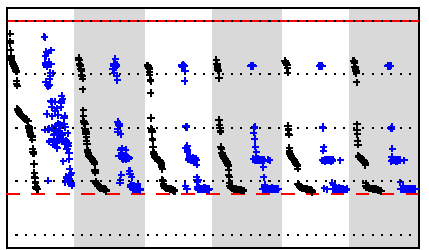
\includegraphics[scale = 1.0]{figs/prioraug/intdiff_heu1.pdf}};
  \node at (0,-2.8) {Algorithm Iteration};
  \node at (-2.9,-2.35) {1};
  \node at (-1.74,-2.35) {2};
  \node at (-0.58,-2.35) {3};
  \node at (0.58,-2.35) {4};
  \node at (1.74,-2.35) {5};
  \node at (2.9,-2.35) {6};
  \node[rotate=90] at (-3.85,0) {Cost};
  \node at (-3.85,1.75) {1.0};
  \node at (-3.85,-1.8) {0.2};
  \node[sum,red,line width=1.8pt] at (2.88,1.0) {};
  \node[sum,black,line width=1.8pt] at (2.88,-0.6) {};
  \node[sum,blue,line width=1.8pt] at (2.88,-1.1) {};
  \node at (0,-2.5) {};
\end{tikzpicture}
\label{fig:standi1}
}
\hspace{1cm}
\subfigure[Three locally optimal solutions]{
\begin{tikzpicture}
  \node at (0,0) {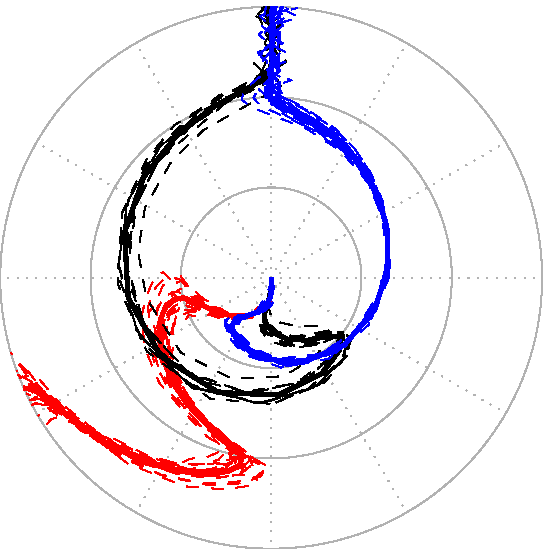
\includegraphics[scale = 0.5]{figs/prioraug/nifty.pdf}};
  \node at (0.65,0.65) {\footnotesize 1$\,$s};
  \node at (1.25,1.25) {\footnotesize 2$\,$s};
  \node at (1.79,1.79) {\footnotesize 3$\,$s};
  \node at (0,-2.55) {down};
  \node at (0,2.55) {upright};
\end{tikzpicture}
\label{fig:standj1}
}
\caption{The graph in (a) depicts the cost trajectories over six iterations of 50 Monte Carlo runs of the standard learning algorithm to the pendulum problem. The black crosses show the actual costs incurred and the blue crosses show the associated mean predicted costs. The maximum cost and the global optimum are shown by the red line and the red dashed line respectively. The three solutions that the algorithm tended to settle for are shown by the trajectories in (b). The blue is close the global optimum solution, consisting of a single swing-back, while the black is a local optimum consisting of two swings. Finally, the red is a locally optimal solution of simply applying full actuation torque over the whole horizon.}
\label{fig:stand1}
\end{figure}
%-------------------------------------------------------------------------------------------------------------------------------------------




\subsubsection{Standard Method}
The results of applying the learning algorithm of \cite{DR11}, which we shall refer to as the ``standard method", to the pendulum are shown in \Fig{standi1}. This is clearly a relatively easy task in terms of system identification since the predicted costs match the actual costs after only two iterations (6$\,$s of data). In terms of learning the control task, many of the runs can learn a policy that works after just the first iteration (3$\,$s of data) while the majority of runs achieve the swing up task by the second iteration.

What makes this an interesting problem is not the learning speed but that there are clearly three solutions in which the algorithm gets stuck. Note that the algorithm was run as long as 10 iterations and the distribution of solutions did not change. The three locally optimal solutions are shown in \Fig{standj1}. The first, shown in blue, is an ideal solution consisting of a single-swing back before the swing-up. This is close to the theoretical limit, shown by the dashed red line.
% and determined through dynamic programming. 
It is desirable for all runs to end up here. The second mode, shown in black, is a locally optimal solution consisting of two swings before the swing-up. Finally, there is a common failure mode shown in red in which the policy simply applies the maximum control action over the whole horizon and gets stuck here.








%-------------------------------------------------------------------------------------------------------------------------------------------
\begin{figure*}
\centering \footnotesize
\subfigure[Use GPs to learn evolution of both $\theta$ and $\dot\theta$.]{ % Uncertainty in theta
\begin{tikzpicture}
  \node at (5.2,0) {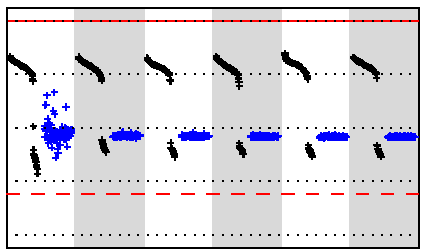
\includegraphics[scale = 0.7]{figs/prioraug/addnoise1.pdf}};
  \node at (0,0) {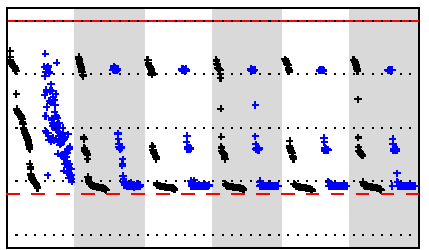
\includegraphics[scale = 0.7]{figs/prioraug/addnoise2.pdf}};
  \node at (-5.2,0) {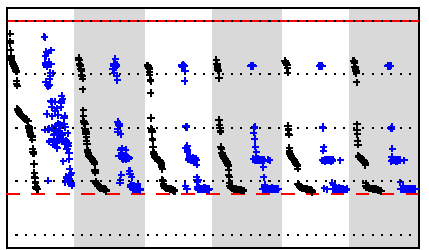
\includegraphics[scale = 0.7]{figs/prioraug/intdiff_heu1.pdf}};
  \node[rotate=90] at (-8.0,0) {Cost};
  \node at (-8.0,1.25) {1.0};
  \node at (-8.0,-1.25) {0.2};
  \node[fill=white,rounded corners] at (-3.5,-1.15) {\scriptsize $\sigma^2 = 0$};
  \node[fill=white,rounded corners] at (1.6,-1.15) {\scriptsize $\sigma^2 = 0.01$};
  \node[fill=white,rounded corners] at (6.85,-1.15) {\scriptsize $\sigma^2 = 0.1$};
\end{tikzpicture}
\label{fig:noisy1}
} 
\subfigure[Reconstruct $\theta$ using the Euler method.]{ % Uncertainty in dtheta
\begin{tikzpicture}
  \node at (5.2,0) {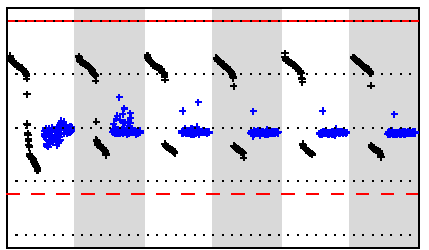
\includegraphics[scale = 0.7]{figs/prioraug/intdiff_eul2.pdf}};
  \node at (0,0) {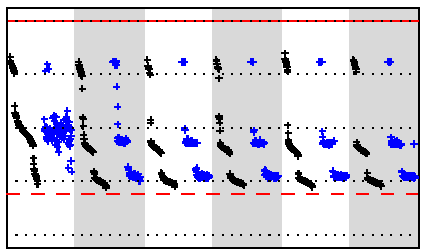
\includegraphics[scale = 0.7]{figs/prioraug/intdiff_eul3.pdf}};
  \node at (-5.2,0) {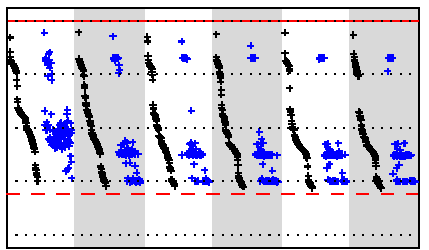
\includegraphics[scale = 0.7]{figs/prioraug/intdiff_eul5.pdf}};
  \node[rotate=90] at (-8.0,0) {Cost};
  \node at (-8.0,1.25) {1.0};
  \node at (-8.0,-1.25) {0.2};
  \node[fill=white,rounded corners] at (-3.5,-1.15) {\scriptsize $\sigma^2 = 0$};
  \node[fill=white,rounded corners] at (1.6,-1.15) {\scriptsize $\sigma^2 = 0.01$};
  \node[fill=white,rounded corners] at (6.85,-1.15) {\scriptsize $\sigma^2 = 0.1$};
\end{tikzpicture}
\label{fig:eul1}
}
\subfigure[Reconstruct $\theta$ using the Heun method.]{ % Uncertainty in dtheta
\begin{tikzpicture}
  \node at (5.2,0) {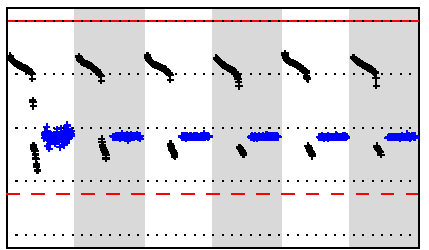
\includegraphics[scale = 0.7]{figs/prioraug/intdiff_heu2.pdf}};
  \node at (0,0) {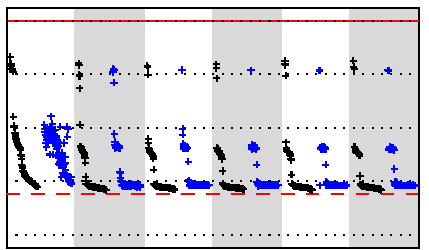
\includegraphics[scale = 0.7]{figs/prioraug/intdiff_heu3.pdf}};
  \node at (-5.2,0) {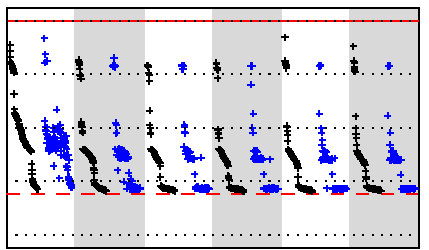
\includegraphics[scale = 0.7]{figs/prioraug/intdiff_heu5.pdf}};
  \node[rotate=90] at (-8.0,0) {Cost};
  \node at (-8.0,1.25) {1.0};
  \node at (-8.0,-1.25) {0.2};
  \node[fill=white,rounded corners] at (-3.5,-1.15) {\scriptsize $\sigma^2 = 0$};
  \node[fill=white,rounded corners] at (1.6,-1.15) {\scriptsize $\sigma^2 = 0.01$};
  \node[fill=white,rounded corners] at (6.85,-1.15) {\scriptsize $\sigma^2 = 0.1$};
\end{tikzpicture}
\label{fig:heu1}
}
\subfigure[Reconstruct $\theta$ using the Cubic method.]{ % Uncertainty in dtheta
\begin{tikzpicture}
  \node at (5.2,0) {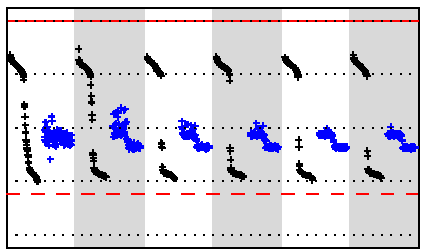
\includegraphics[scale = 0.7]{figs/prioraug/intdiff_fan2.pdf}};
  \node at (0,0) {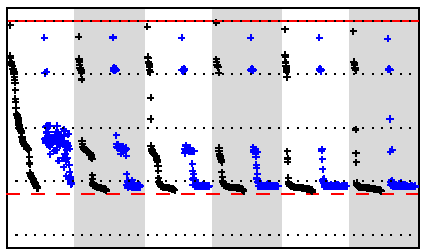
\includegraphics[scale = 0.7]{figs/prioraug/intdiff_fan3.pdf}};
  \node at (-5.2,0) {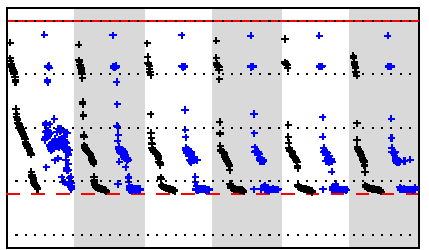
\includegraphics[scale = 0.7]{figs/prioraug/intdiff_fan5.pdf}};
  \node[rotate=90] at (-8.0,0) {Cost};
  \node at (-8.0,1.25) {1.0};
  \node at (-8.0,-1.25) {0.2};
  \node[fill=white,rounded corners] at (-3.5,-1.15) {\scriptsize $\sigma^2 = 0$};
  \node[fill=white,rounded corners] at (1.6,-1.15) {\scriptsize $\sigma^2 = 0.01$};
  \node[fill=white,rounded corners] at (6.85,-1.15) {\scriptsize $\sigma^2 = 0.1$};
\end{tikzpicture}
\label{fig:cub1}
}
\caption{Plots of the distribution of actual costs (black) and the mean predicted cost (blue) for different levels of additive noise $\cN(\bO,\sigma^2\bI)$ on the prediction of $\theta$. The x-axis displays the algorithm iteration and the y-axis shows the cost $J(\bpsi)$. These plots were constructed from 100 Monte Carlo runs with initial training data sets obtained by applying different random torque actions.}
\label{fig:integ}
\end{figure*}
%-------------------------------------------------------------------------------------------------------------------------------------------








\subsubsection{Position Reconstruction}
The explicit inclusion of approximate position-velocity information in the pendulum swing-up problem shall now be considered. The results of applying various position reconstruction schemes are shown in \Fig{integ}. The schemes considered shall be referred to as the Euler, Heun and Cubic methods and consist of the following equations respectively
\begin{align}
\theta_k &= \theta_{k-1} + \Dt\dot\theta_k + \epsilon_k
\label{eqn:pen_eul} \\
\theta_k &= \theta_{k-1} + \tfrac{1}{2}\Dt\big(\dot\theta_k + \dot\theta_{k-1} \big) + \epsilon_k
\label{eqn:pen_heu} \\
\theta_k &= \theta_{k-2} + \tfrac{1}{3}\Dt \big( \dot\theta_{k} + 4\dot\theta_{k-1} + \dot\theta_{k-2} \big) + \epsilon_k
\label{eqn:pen_cub} 
\end{align}
The additive noise term $\epsilon_k \sim \cN(0,\sigma^2)$ is used to encode uncertainty in the approximation scheme. We use values of $\sigma^2=0.01$ and $\sigma^2=0.1$, which correspond to standard deviations of around $6^\circ$ and $18^\circ$ respectively. The Euler and Heun methods are so called because of their similarity to the Euler and Heun methods for numerical integration. Note that it is unnecessary to predict differences because we are not learning the relationship. 
%
\Tab{integ} gives some additional statistics of the learned policies at the end of the six iterations for $\sigma^2=0$ and $\sigma^2=0.01$. It shows how many runs ended up in the bad local minimum and the number that ended up in the global optimum solution.


Firstly, observe \Fig{noisy1} which shows the effect of applying additional noise to the Gaussian process prediction of $\theta$. Setting $\sigma^2=0$ clearly reproduces the results of the standard algorithm. An interesting thing happens when the noise level is increased to $\sigma^2=0.01$ and that is that the algorithm converges on its solution much faster, however more runs end up in the failure mode. This additional uncertainty is in some senses equivalent to asking the algorithm to design a policy that is robust to a greater level of uncertainty. At $\sigma^2=0.1$ the noise level is too high for any reliable prediction or learning to take place. However it is interesting to note that it sometime enters a failure mode that involves the pendulum swinging round and round as hard as it can.

Now, consider the results of applying the Euler method in \Eq{pen_eul} to reconstruct $\theta$ at every timestep, shown in \Fig{eul1}. Taking the raw approximation with $\sigma^2=0$ yields much poorer performance than the standard algorithm with only a few of the runs reaching a solution close to the global optimum. The large discrepancy between predicted and actual costs indicate that this approximation is too poor to give reliable performance. Moving up to $\sigma^2=0.01$ an interesting thing occurs. The learning performance is comparable to that of the standard algorithm. Note that the predictions are slightly under-confident. Again, with $\sigma^2=0.1$ the algorithm fails to achieve the task. This points to the fact that a poor approximation method can still work well given an appropriate amount of ``distrust" of the results it is producing.

%-------------------------------------------------------------------------------------------------------------------------------------------
\begin{table}[]
\renewcommand{\arraystretch}{1.3}
\begin{center}
\small
%\setlength{\extrarowheight}{2pt}
\rowcolors{1}{black!10}{white}
\begin{tabular}{ c | cc | cc | cc | cc }
\toprule[1.5pt] 
& \multicolumn{2}{c|}{\bf Standard} & \multicolumn{2}{c|}{\bf Euler} & \multicolumn{2}{c|}{\bf Heun} & \multicolumn{2}{c}{\bf Cubic} \\
$\sigma^2$ & 0 & 0.01 & 0 & 0.01 & 0 & 0.01 & 0 & 0.01 \\
\hline
Failed             & 12 & 17     & 19 & 11        & 7 & 3        & 12 & 8 \\
Suboptimal     & 33 & 16     & 63 & 38        & 38 & 21    & 30 & 3 \\
Optimal           & 55 & 67     & 18 & 51        & 55 & 76    & 58 &  89  \\
\bottomrule[1.5pt]
\end{tabular}
\end{center}
\caption{This table provides the number of learning algorithm runs that have fallen into either the bad local minimum, a suboptimal solution or the global optimum solution at the end of the six trials out of the 100 Monte Carlo runs. They are compared across the different methods for position reconstruction and values of additive predictive noise. The values correspond to those depicted in \Fig{integ}.}
\label{tab:integ}
\end{table}
%-------------------------------------------------------------------------------------------------------------------------------------------


The Heun method with $\sigma^2=0$ performs marginally better than the standard algorithm as shown in \Fig{heu1} and \Tab{integ} with less runs falling into the bad local optimum but the same number finding the global optimum. Moving to a noise level of $\sigma^2=0.01$ we can see that there is actually a marked improvement in performance in terms of the number of runs finding the global optimum and avoiding the bad local minimum. As a side note, the approximation based on a quadratic fit given in \Eq{dada} produced very similar results to the Heun method.
%
Finally, the results of the Cubic method are shown in \Fig{cub1}. The results of noise free application has very similar performance to both the Standard and Heun methods. However, moving to $\sigma^2=0.01$ we see an even greater improvement in performance than observed with the Heun method with nearly 90\% of the runs finding the global optimum solution but with more falling into the bad local optimum.

What can be drawn from these results is that the incorporation of time-derivative prior information can be helpful in avoiding locally optimal solutions to a given control task. But the most interesting feature is that the inclusion of uncertainty, i.e.\ an explicit suspicion of the predictions produced by a prior model, can potentially lead to better performance, or indeed much worse if the uncertainty level is too high.



%-------------------------------------------------------------------------------------------------------------------------------------------
\begin{figure*}
\centering \footnotesize
\subfigure[Use GPs to learn evolution of both $\theta$ and $\dot\theta$.]{ % Uncertainty in theta
\begin{tikzpicture}
  \node at (5.2,0) {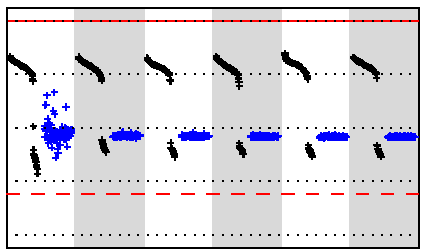
\includegraphics[scale = 0.7]{figs/prioraug/addnoise1.pdf}};
  \node at (0,0) {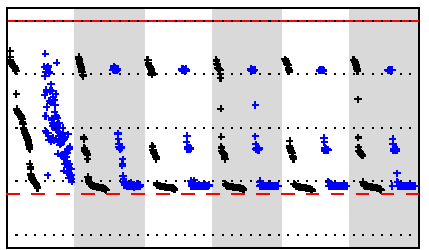
\includegraphics[scale = 0.7]{figs/prioraug/addnoise2.pdf}};
  \node at (-5.2,0) {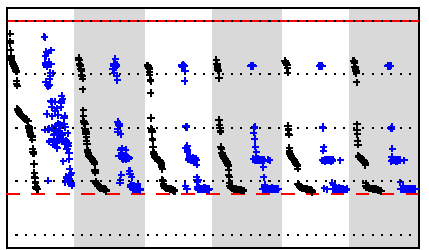
\includegraphics[scale = 0.7]{figs/prioraug/intdiff_heu1.pdf}};
  \node[rotate=90] at (-8.0,0) {Cost};
  \node at (-8.0,1.25) {1.0};
  \node at (-8.0,-1.25) {0.2};
  \node[fill=white,rounded corners] at (-3.5,-1.15) {\scriptsize $\sigma^2 = 0$};
  \node[fill=white,rounded corners] at (1.6,-1.15) {\scriptsize $\sigma^2 = 0.01$};
  \node[fill=white,rounded corners] at (6.85,-1.15) {\scriptsize $\sigma^2 = 0.1$};
\end{tikzpicture}
\label{fig:noisy2}
} 
\subfigure[Reconstruct $\dot\theta$ using the Euler method.]{ % Uncertainty in dtheta
\begin{tikzpicture}
  \node at (5.2,0) {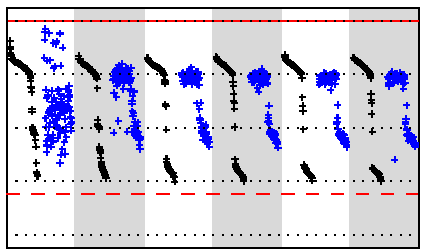
\includegraphics[scale = 0.7]{figs/prioraug/intdiff_eul6.pdf}};
  \node at (0,0) {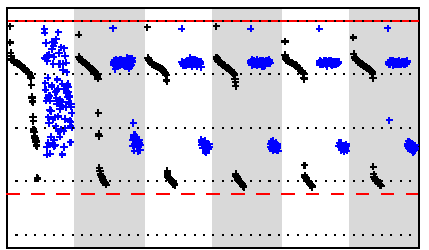
\includegraphics[scale = 0.7]{figs/prioraug/intdiff_eul7.pdf}};
  \node at (-5.2,0) {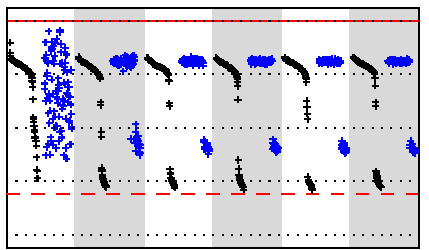
\includegraphics[scale = 0.7]{figs/prioraug/intdiff_eul9.pdf}};
  \node[rotate=90] at (-8.0,0) {Cost};
  \node at (-8.0,1.25) {1.0};
  \node at (-8.0,-1.25) {0.2};
  \node[fill=white,rounded corners] at (-3.5,-1.15) {\scriptsize $\sigma^2 = 0$};
  \node[fill=white,rounded corners] at (1.6,-1.15) {\scriptsize $\sigma^2 = 0.01$};
  \node[fill=white,rounded corners] at (6.85,-1.15) {\scriptsize $\sigma^2 = 0.1$};
\end{tikzpicture}
\label{fig:eul2}
}
\subfigure[Reconstruct $\dot\theta$ using the Heun method.]{ % Uncertainty in dtheta
\begin{tikzpicture}
  \node at (5.2,0) {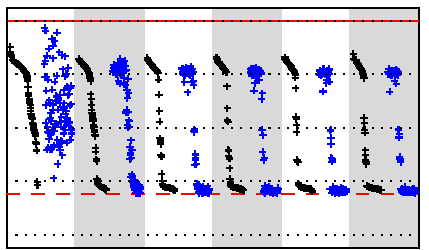
\includegraphics[scale = 0.7]{figs/prioraug/intdiff_heu6.pdf}};
  \node at (0,0) {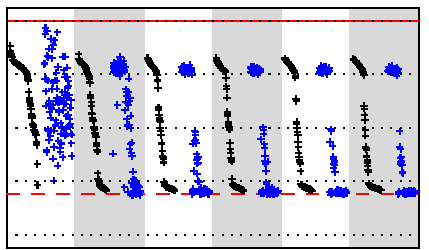
\includegraphics[scale = 0.7]{figs/prioraug/intdiff_heu7.pdf}};
  \node at (-5.2,0) {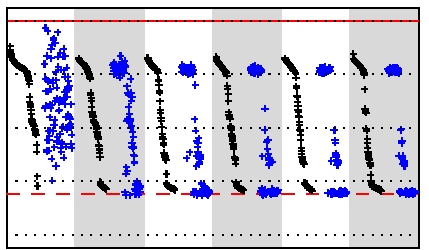
\includegraphics[scale = 0.7]{figs/prioraug/intdiff_heu9.pdf}};
  \node[rotate=90] at (-8.0,0) {Cost};
  \node at (-8.0,1.25) {1.0};
  \node at (-8.0,-1.25) {0.2};
  \node[fill=white,rounded corners] at (-3.5,-1.15) {\scriptsize $\sigma^2 = 0$};
  \node[fill=white,rounded corners] at (1.6,-1.15) {\scriptsize $\sigma^2 = 0.01$};
  \node[fill=white,rounded corners] at (6.85,-1.15) {\scriptsize $\sigma^2 = 0.1$};
\end{tikzpicture}
\label{fig:heu2}
}
\caption{Plots of the distribution of actual costs (black) and the mean predicted cost (blue) for different levels of additive noise $\cN(\bO,\sigma^2\bI)$ on the prediction of $\dot\theta$. The x-axis displays the algorithm iteration and the y-axis shows the cost $J(\bpsi)$. These plots were constructed from 100 Monte Carlo runs with initial training data sets obtained by applying different random torque actions.}
\label{fig:differ}
\end{figure*}
%-------------------------------------------------------------------------------------------------------------------------------------------




\subsubsection{Velocity Reconstruction}
Now consider the use of velocity reconstruction to obtain predictions for $\dot\theta$ based on GP predictions of $\theta$. The Euler and Heun equations in this case are given by
\begin{align}
\dot\theta_k &= \Dt\inv\big(\theta_k - \theta_{k-1}\big) + \epsilon_k
\label{eqn:pen_eulv} \\
\dot\theta_k &= 2\Dt\inv\big(\theta_k - \theta_{k-1} \big) - \dot\theta_{k-1} + \epsilon_k
\label{eqn:pen_heuv}
\end{align}
respectively. We again use noise variances of $\sigma^2=0.01$ and $\sigma^2=0.1$, which correspond, in this case, to standard deviations of $0.1\,$rad$\,$s$\inv$ and $0.316\,$rad$\,$s$\inv$ respectively. Higher order approximations have not actually been considered here since applying them to this problem led to an explosion in the covariance of the predicted state at later timesteps and therefore numerically unstable results. This occurred because the variance in the initial estimates of $\theta$ was quite large, but this uncertainty was then amplified many times since the coefficients of the linear model were relatively large.

The results of the Euler and Heun approximation schemes are given in \Fig{differ}. It is quite clear from these plots that the use of velocity reconstruction leads to much poorer performance than the standard algorithm in all cases. The Euler results shown in \Fig{eul2} fail in almost all the runs and the discrepancy between the predicted and actual costs is large. However, even in the face of such a poor approximation, some of the runs are still able to solve the task.

The effect of additional uncertainty when using a Heun approximation leads to progressively improved results with the best performance achieved when $\sigma^2=0.1$. Increasing noise appears to have the effect of stopping the runs falling into ``weak" local minima such as the two-swing solution and polarises the results into the ``strong" minima of the global optimum and the failure mode.



%-------------------------------------------------------------------------------------------------------------------------------------------
\begin{figure}
\centering \small
\begin{tikzpicture}
  \node at (5.2,0) {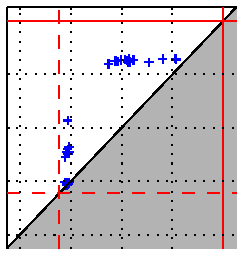
\includegraphics[scale = 1.2]{figs/prioraug/penpred3.pdf}};
  \node at (0,0) {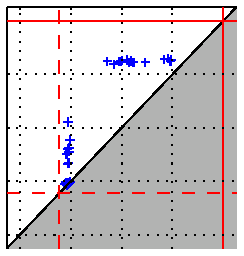
\includegraphics[scale = 1.2]{figs/prioraug/penpred2.pdf}};
  \node at (-5.2,0) {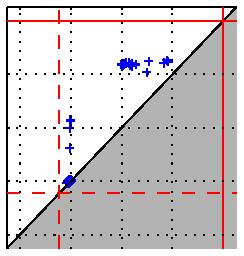
\includegraphics[scale = 1.2]{figs/prioraug/penpred1.pdf}};
  \node[rotate=90] at (-7.95,0) {Predicted Cost};
  \node at (-7.95,2.2) {1.0};   \node at (7.3,-2.85) {1.0};
  \node at (-7.95,-2.15) {0.2};   \node at (-7.3,-2.85) {0.2};
  \node[] at (0,-2.85) {Lowest Predicted Cost using a Globally Optimal Policy};
  \node[fill=white,draw,rounded corners] at (-5.2,-1.9) {$\sigma^2 = 0.10$};
  \node[fill=white,draw,rounded corners] at (0,-1.9) {$\sigma^2 = 0.01$};
  \node[fill=white,draw,rounded corners] at (5.2,-1.9) {$\sigma^2 = 0.00$};
\end{tikzpicture}
\caption{These plots are directly related to the Monte Carlo runs shown in \Fig{heu2} in which a Heun-type method has been used to achieve velocity reconstruction. They show the lowest predicted cost predicted by a given internal model for a globally optimal policy against the policy the algorithm actually converged on using this model. Points appearing in the gray region would indicate that the model was predicting that the globally optimal solution was performing worse than its own solution.}
\label{fig:penpred}
\end{figure}
%-------------------------------------------------------------------------------------------------------------------------------------------



An important question to be raised is why does velocity reconstruction perform so much poorer than position reconstruction. It is evidently not due to the predictive quality of the predictions since for the Heun method these are clearly quite accurate. To investigate this phenomenon a further study was carried out on the Heun Monte Carlo runs shown in \Fig{heu2}. The learned model at the end of the sixth iteration for every run was taken and every policy which achieved the globally optimal solution was evaluated with respect to this model to see whether the policy it had converged on was genuinely optimal with respect to the learned model or whether the algorithm had simply got stuck in a local minimum. The results are shown in \Fig{penpred}. Clearly the problem here is that the use of velocity reconstruction in the pendulum problem produces a problem with stronger local minima than with position reconstruction.

The reason for this strange behaviour could be due to the fact that the dynamics of position variables tend to be slower than the associated velocity. This is because integration in time has a low-pass filtering effect. Therefore, trying to reconstruct the quickly varying dynamics from the slowly varying ones has more potential for erroneous results. 



\subsubsection{Computational Savings}


%-------------------------------------------------------------------------------------------------------------------------------------------
\begin{figure}[t!]
\centering \small
\begin{tikzpicture}
  \node at (0,0) {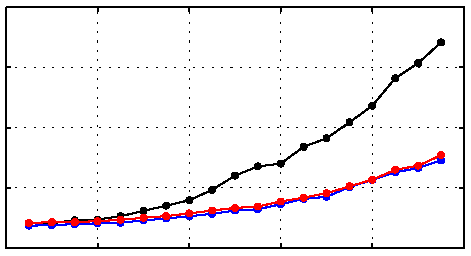
\includegraphics[scale=1.1]{figs/prioraug/pen_timing.pdf}};
  \node[rotate=90] at (-4.75,0) {CPU time (s)};
  \node[anchor=east] at (-4.3,2.2) {20};   \node[anchor=east] at (-4.3,-2.2) {0};
  \node at (0,-2.6) {Training data set size};
  \node at (-4.2,-2.55) {0};  \node at (4.2,-2.55) {500};
\end{tikzpicture}
\caption{Comparison of CPU time for a single cost function evaluation (with derivatives) for the pendulum. The black line is for the prediction of $\theta$ and $\dot\theta$ using two GPs. The blue line is for the case where one of the states is reconstructed using information back to time $k-1$ and the red line for information back to $k-2$. The x-axis depicts the size of training data set available to the GP.}
\label{fig:pencomps}
\end{figure}
%-------------------------------------------------------------------------------------------------------------------------------------------



One of the major advantages of using prior information in this way is the computational savings in prediction and cost function evaluation. Since we are removing one of the two Gaussian process models (for both position and velocity reconstruction) and replacing it with a linear mapping we expect the computation time to be approximately halved. \Fig{pencomps} shows a plot of the CPU time required to evaluate $J(\bpsi)$ (and its derivatives with respect to policy parameters) against the size of the training data set available to the GP. Below about $n=100$ there is no significant difference between the three except that it costs slightly more to include the delayed states for approximations based on information at time $k-2$. However, beyond $n=200$ the computational savings are significant, with the inclusion of delayed states coming at essentially no extra cost. The trends do indeed show a linear saving in the number of GPs we can replace with linear mappings.









\subsection{Example: Unicycle} \label{sec:unicycle}








%-------------------------------------------------------------------------------------------------------------------------------------------
%\begin{figure}[t]
%\centering
%\subfigure[Robotic unicycle]{
%
\begin{tikzpicture}[]

\begin{scope}[canvas is xz plane at y=-1.5]
  \draw[draw=black,fill=black!10,rounded corners] (2.3,2) rectangle (-2.5,-2);
\end{scope}

% origin is (-2.5,-1.5,2)
\draw[thick,blue,-latex'] (-2.7,-1.5,2) -- (-0.5,-1.5,2);
\draw[thick,blue,-latex'] (-2.5,-1.7,2) -- (-2.5,0.5,2);
\draw[thick,blue,-latex'] (-2.5,-1.5,2.3) -- (-2.5,-1.5,-0.8);

\begin{scope}[canvas is xz plane at y=-0.1]
  \draw[rotate=0,-latex',black, thick] (-2.2,2) arc (0:-320:0.3cm);
\end{scope}
\begin{scope}[canvas is xy plane at z=0.1]
  \draw[rotate=0,-latex',black, thick] (-2.25,-1.5) arc (0:-300:0.25cm);
\end{scope}
\begin{scope}[canvas is yz plane at x=-1.1]
  \draw[rotate=0,-latex',black, thick] (-1.2,2) arc (0:300:0.3cm);
\end{scope}

\begin{scope}[canvas is yx plane at z=-0.05]
  \draw[draw=black,fill=black!30,thick,opacity=0.8] (0,0) circle (1.5cm);
\end{scope}
\begin{scope}[canvas is yx plane at z=0.05]
  \draw[draw=black,fill=black!30,thick,opacity=0.8] (0,0) circle (1.5cm);
  \draw[draw=black,fill=black,thick] (0,0) circle (0.1cm);
  \draw[rotate=45,-latex',red, thick] (1.7,0) arc (0:50:1.7cm);
  \draw[rotate=45,-latex', thick] (0.3,0) arc (0:300:0.3cm);
\end{scope}

\draw[line width = 0.05cm] (0,3,0) -- (0,0,0);
\draw[line width = 0.1cm] (0,3,0) -- (0,1.48,0);

\begin{scope}[canvas is xz plane at y=2.94]
  \draw[draw=black,fill=black!30,thick,opacity=0.8] (0,0) circle (1.5cm);
\end{scope}
\begin{scope}[canvas is xz plane at y=3]
  \draw[draw=black,fill=black!30,thick,opacity=0.8] (0,0) circle (1.5cm);
  \draw[draw=black,fill=black,thick] (0,0) circle (0.1cm);
   \draw[rotate=-5,-latex',red, thick] (1.7,0) arc (0:-50:1.7cm);
   \draw[rotate=0,-latex', thick] (0.4,0) arc (0:-300:0.4cm);
\end{scope}


\node at (-0.4,-1.5,2.8) {{\color{blue}$x$}}; \node at (-0.9,-1.2,1.7) {$\theta$};
\node at (-2.1,-1.5,-0.2) {{\color{blue}$y$}}; \node at (-2.5,-1.0,-0.2) {$\phi$};
\node at (-2.2,0.4,2) {{\color{blue}$z$}}; \node at (-2.9,0.2,2) {$\psi$};

\node at (-0.3,-0.6,0) {$\phi_\text{w}$}; \node at (-0.7,3,0.3) {$\psi_\text{t}$};
\node at (1.9,0.7,0) {\color{red}$u_\text{w}$}; \node at (2.3,3.4,0.5) {\color{red}$u_\text{t}$};


\end{tikzpicture}
%\label{fig:unicycle}
%}
%\hspace{1cm}
%\subfigure[Body centred coordinates]{
%\begin{tikzpicture}
%  \draw[draw=black,fill=black!10,rounded corners] (-3,-3) rectangle (3,3);
%
%  \draw[thick,blue,-latex']  (1,0.9) -- (1,2.5);
%  \draw[thick,blue,-latex']  (0.9,1) -- (2.5,1);
%  \draw[thick,red,fill=red] (1,1) circle (0.06cm);
%  
%  \draw[rotate=50,thick, fill=black!30] (-1.3,0) circle (1cm);
%  \draw[rotate=50,thin] (-1.33,-1) -- (-1.33,1);
%  \draw[rotate=50,thin] (-1.27,-1) -- (-1.27,1);
%  \draw[rotate=50,thick,blue,-latex'] (-1.3,0.1) -- (-1.3,-1.5);
%  \draw[rotate=50,thick,blue,-latex'] (-1.4,0) -- (0.2,0.1);
%  
%  \node at (-0.2,1.3) {\footnotesize origin};
%  \draw[thin,black,-latex']  (0.3,1.3) -- (0.9,1.05);
%  \node at (0.0,-2.0) {\color{blue}$x_c$};
%  \node at (0.2,-0.1) {\color{blue}$y_c$};
%  \node at (2.2,0.75) {\color{blue}$x$};
%  \node at (1.25,2.2) {\color{blue}$y$};
%  
%\end{tikzpicture}
%\label{fig:unicycle2}
%}
%\caption{Robotic unicycle with roll angle $\theta$, pitch angle $\phi$, yaw angle $\psi$, turntable angle $\psi_{\text{t}}$ and wheel angle $\phi_{\text{w}}$. The controlled inputs are the torque applied to the turntable $u_{\text{t}}$ and the torque applied to the wheel $u_{\text{w}}$.}
%\end{figure}
%-------------------------------------------------------------------------------------------------------------------------------------------








\subsubsection{Setup}
The scheme was then tested on a highly nontrivial control problem: balancing a simulated robotic unicycle. The layout of this problem is shown in \Fig{unicycle}. What makes this such a hard problem is that the rolling motion of the unicycle can only be affected indirectly through application of a torque to the turntable on top of the unicycle. The equations of motion for this system were derived by \cite{For09} and can be found in \App{unicycle}, along with a full derivation. 

The state is given by $\bx = [\phi, \dot\phi, \theta, \dot\theta, \psi, \dot\psi, \dot\phi_\te{w}, \dot\psi_\text{t},x_\text{c}, y_\text{c}]^\top \in \RR^{10}$ with pitch angle $\phi$, roll angle $\theta$, yaw angle $\psi$, wheel angle $\phi_\te{w}$, turntable angle $\psi_\te{t}$ and the location of the origin $(x_\te{c},y_\te{c})$ with respect to a body-fixed reference frame. These are depicted in \Fig{unicycle}. We note that the dynamics are clearly independent of $\phi_\te{w}$ and $\psi_\te{t}$ for a wheel and turntable with uniform radial distribution of mass.  The constrained action vector is $\bu = [u_\te{w}, u_\te{t}]^\top \in \RR^2$, where $u_\te{w}$ is the torque applied to the wheel and $u_\te{t}$ is the torque applied to the turntable.

The policy itself was an affine policy $\bu = \bK\bx + \bk$ with gain matrix $\bK$ and offset $\bk$. Note that the distinction between these terms and the covariance matrix of a GP will be clear from the context. The discrete timestep was set to $\Dt = 0.15\,$s. This is a large timestep given the dynamics of the unicycle and therefore makes the task of control relatively hard. However, a long timestep is necessary to ensure the policy learning time is not in the order of weeks.


%-------------------------------------------------------------------------------------------------------------------------------------------
\begin{figure}
\centering
%set the plot display orientation
%synatax: \tdplotsetdisplay{\theta_d}{\phi_d}
\tdplotsetmaincoords{65}{100}

%define polar coordinates for some vector
%TODO: look into using 3d spherical coordinate system
\pgfmathsetmacro{\magW}{4}
\pgfmathsetmacro{\psiW}{-30}
\pgfmathsetmacro{\theW}{10}
\pgfmathsetmacro{\phiW}{15}

%start tikz picture, and use the tdplot_main_coords style to implement the display 
%coordinate transformation provided by 3dplot
\footnotesize
\begin{tikzpicture}[scale=0.95,tdplot_main_coords]

%set up some coordinates ... GET FROM MATLAB
%-----------------------
\coordinate (O) at (1.7321,-1,0);
\coordinate (B) at (2.5,4.3301,0);
\coordinate (Bp) at (4.2321,3.3301,0);
\coordinate (W) at (2.7256,4.1999,1.4772);
\coordinate (Wt) at (3.1767,3.9394,4.4316);
\coordinate (Wtp) at (2.7256,4.1999,4.4316);
\coordinate (Wbp) at (2.7256,4.1999,0);
\coordinate (T) at (2.7969,2.8138,5.7578);
\coordinate (F) at (2.7612,3.5069,3.6175);

%draw figure contents
%--------------------

%draw the main coordinate system axes
\tdplotsetrotatedcoordsorigin{(O)}
\tdplotsetrotatedcoords{0}{0}{0}
\draw[tdplot_rotated_coords,-latex,blue,thick] (0,0,0) -- (1.5,0,0) node[anchor=south east]{$\bi$};
\draw[tdplot_rotated_coords,-latex,blue,thick] (0,0,0) -- (0,1.5,0) node[anchor=south]{$\bj$};
\draw[tdplot_rotated_coords,-latex,blue,thick] (0,0,0) -- (0,0,1.5) node[anchor=south]{$\bk$};
\draw[dashed] (W) -- (Wt);
\draw[dashed] (Wtp) -- (Wbp);
\draw[dashed] (B) -- (W);

\draw[red,-latex] (B) -- (Bp);
\draw[red,-latex] (Bp) -- (O);
\node at (0,0.8,-1.7) {\color{red} $x_\te{c}$};
\node at (0,3.2,-1.4) {\color{red} $y_\te{c}$};
\tdplotsetrotatedcoords{\psiW}{0}{0}
\tdplotsetrotatedcoordsorigin{(Bp)}
\draw[tdplot_rotated_coords,very thin] (-0.35,0,0) -- (-0.35,-0.35,0) -- (0,-0.35,0);


% draw frame
\draw[very thick,black] (W) -- (T);
\tdplotsetrotatedcoords{\psiW}{100}{0}
\tdplotsetrotatedcoordsorigin{(F)}
\draw[tdplot_rotated_coords,fill=black] (0,0,0) circle (0.12);

% draw turntable
\tdplotsetrotatedcoords{\psiW}{\theW}{\phiW}
\tdplotsetrotatedcoordsorigin{(T)}
\draw[tdplot_rotated_coords,very thick,fill=black,fill opacity=0.2] (0,0,0) circle (1.5);
\draw[tdplot_rotated_coords,fill=black] (0,0,0) circle (0.12);
\tdplotdrawarcarrow[tdplot_rotated_coords,red]{(T)}{0.65}{0}{270}{}{}
\tdplotdrawarcarrow[tdplot_rotated_coords,blue]{(T)}{0.4}{0}{270}{}{}
\node at (0,3.25,4.8) {\color{red} $\psi_\te{t}$};
\node at (0,1.7,4.2) {\color{blue} $u_\te{t}$};

% draw wheel
\tdplotsetrotatedcoords{\psiW}{100}{0} % add 90 to j angle
\tdplotsetrotatedcoordsorigin{(W)}
\draw[tdplot_rotated_coords,very thick,fill=black,fill opacity=0.2] (0,0,0) circle (1.5);
\draw[tdplot_rotated_coords,fill=black] (0,0,0) circle (0.12);
\tdplotdrawarcarrow[tdplot_rotated_coords,red]{(W)}{0.6}{0}{270}{}{}
\tdplotdrawarcarrow[tdplot_rotated_coords,blue]{(W)}{0.4}{0}{270}{}{}
\node at (0,4.35,0.5) {\color{red} $\phi_\te{w}$};
\node at (0,3.3,-0.1) {\color{blue} $u_\te{w}$};



% show theta and phi
\tdplotdrawarcarrow[red]{(O)}{0.8}{0}{60}{anchor=north}{\color{red} $\psi$}
\tdplotsetrotatedcoords{\psiW}{190}{-90} % add 180 to j angle
\tdplotsetrotatedcoordsorigin{(W)}
\tdplotdrawarcarrow[tdplot_rotated_coords,red]{(W)}{2.8}{80}{90}{anchor=south}{\color{red} $\theta$}
\tdplotsetrotatedcoords{\psiW}{100}{0} % add 90 to j angle
\tdplotsetrotatedcoordsorigin{(W)}
\tdplotdrawarcarrow[tdplot_rotated_coords,red]{(W)}{2.8}{180}{195}{anchor=south}{\color{red} $\phi$}


\end{tikzpicture}
\caption{The robotic unicycle. The spatial position of the unicycle is defined by the pitch angle $\phi$, roll angle $\theta$, yaw angle $\psi$, wheel angle $\phi_\te{w}$, turntable angle $\psi_\te{t}$ and the body-centred coordinates of the global origin $(x_\te{c},y_\te{c})$. The controlled inputs are the motor torque applied to the wheel $u_\te{w}$ and the motor torque applied to the turntable $u_\te{t}$.}
\label{fig:unicycle}
\end{figure}
%-------------------------------------------------------------------------------------------------------------------------------------------




%-------------------------------------------------------------------------------------------------------------------------------------------
\begin{figure}
\centering \footnotesize
\subfigure[GP models for all states]{ % Uncertainty in theta
\begin{tikzpicture}
  \node at (0,0) {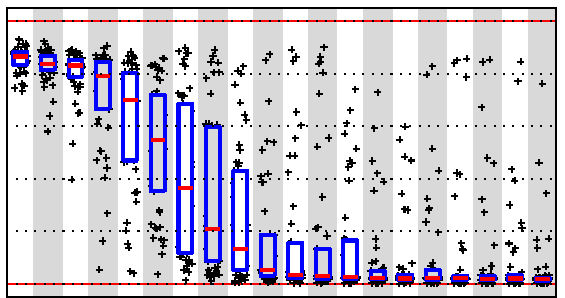
\includegraphics[scale = 0.75]{figs/prioraug/uniplotY1.pdf}};
  \node[rotate=90] at (-3.75,0) {Cost};
  \node at (-3.7,1.6) {1}; \node at (-3.7,-1.7) {0};
\end{tikzpicture}
\label{fig:uni_sta}
}
\subfigure[Reconstruct $\phi, \theta$ and $\psi$ using the Euler method]{ % Uncertainty in theta
\begin{tikzpicture}
  \node at (0,0) {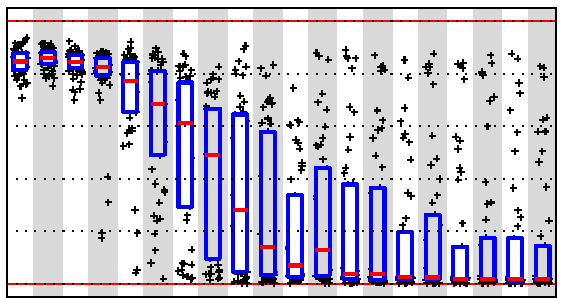
\includegraphics[scale = 0.75]{figs/prioraug/uniplotY2.pdf}};
  \node[rotate=90] at (-3.75,0) {Cost};
  \node at (-3.7,1.6) {1}; \node at (-3.7,-1.7) {0};
\end{tikzpicture}
\label{fig:uni_eul}
}
\subfigure[Reconstruct $\phi, \theta$ and $\psi$ using the Heun method]{ % Uncertainty in theta
\begin{tikzpicture}
  \node at (0,0) {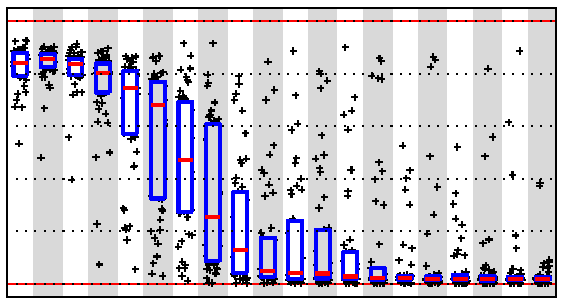
\includegraphics[scale = 0.75]{figs/prioraug/uniplotY3.pdf}};
  \node[rotate=90] at (-3.75,0) {Cost};
  \node at (-3.7,1.6) {1}; \node at (-3.7,-1.7) {0};
\end{tikzpicture}
\label{fig:uni_heu}
}
\subfigure[Reconstruct $\phi, \theta$ and $\psi$ using the Cubic method]{ % Uncertainty in theta
\begin{tikzpicture}
  \node at (0,0) {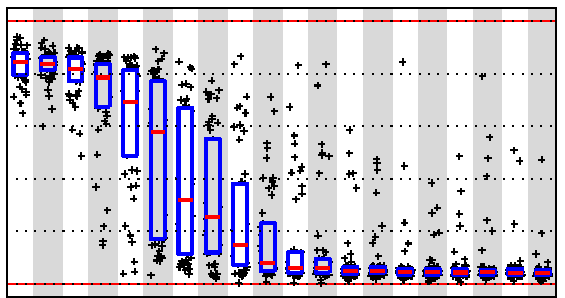
\includegraphics[scale = 0.75]{figs/prioraug/uniplotY5.pdf}};
  \node[rotate=90] at (-3.75,0) {Cost};
  \node at (-3.7,1.6) {1}; \node at (-3.7,-1.7) {0};
\end{tikzpicture}
\label{fig:uni_fan}
}
\caption{Boxplots depicting the cost $J(\bpsi)$ of applying the learned control policy after a given iteration of the algorithm. These were constructed from 50 Monte Carlo runs with random initial training data sets of around 10$\,$s. The blue box encloses the 25$\tth$ to 75$\tth$ percentile of the data, with the 50$\tth$ percentile shown by the red line.}
\label{fig:uniplots}
\end{figure}
%-------------------------------------------------------------------------------------------------------------------------------------------





The state measurement was corrupted with uncorrelated Gaussian white noise. Realistic values for the standard deviation of the noise on each state are around $0.01\,$rad for the roll angle, $0.03\,$rad for all other angles, $0.03\,$rad$\,$s$\inv$ for the angular velocities and $3\,$cm for the coordinates states. With this level of noise, the learning task is too hard for the algorithm since the Gaussian processes overestimate the noise variance significantly. This is because a standard assumption of GP modelling is that the input training data is noise free. This issue has been addressed by \cite{MR11} who provide a method called Noisy Input Gaussian Processes (NIGP) which takes account of noise on the inputs during training. Using the NIGP method within the learning algorithm, it is able to learn how to balance the unicycle with this level of noise. However, it is unclear at this stage how to combine NIGP with the multiple dynamics models framework. Therefore we consider a problem in which the standard deviation of the noise on measurements of the angles and positions is reduced by a factor of ten.

The control task was to balance the unicycle at the origin $(x_\te{c},y_\te{c}) = (0,0)$ given an initial position drawn from a Gaussian distribution $x_\te{c},y_\te{c} \sim \cN(0,0.01\bI)$, i.e.\ a standard deviation of 10$\,$cm in both $x_\te{c}$ and $y_\te{c}$. We use an inverted-Gaussian stage-cost very similar to one derived by \cite{DHR11}. The stage-cost is of the form
\begin{equation}
c(\bx) = 1 - \exp\Big(-\tfrac{1}{2}d(\bx)^2\Big)
\label{eqn:unicost}
\end{equation}
where $d(\bx)^2$ is the squared distance from the top of the unicycle to the upright position over the origin. In particular this term is given by $d(\bx)^2 = d_x^2 + d_y^2 + d_z^2$ with components
\begin{align*}
d_x &= x_\te{c} - r\sin\phi \\
d_y &= y_\te{c} - (r+r_\te{w})\sin\theta \\
d_z &= (r+r_\te{w}) - (r_\te{w} + r\cos\phi)\cos\theta
\end{align*}
where $r$ is the unicycle frame length and $r_\te{w}$ is the radius of the wheel. The expectation of this stage-cost can be evaluated in exactly the same way as the standard inverted-Gaussian cost by first augmenting the state space with $\sin\phi, \sin\theta, \cos\theta, \cos(\theta+\phi)$ and $\cos(\theta-\phi)$. 
%
We note that the stage-cost we used was tuned slightly in order to penalise the runs in which the unicycle falls over more heavily. Specifically, deviations in the vertical were penalised more than deviations in the horizontal by using $d(\bx)^2 = \tfrac{1}{2}\big(d_x^2 + d_y^2 + (4d_z)^2\big)$. This encodes the fact that falling over is a more serious deviation than being far away horizontally, since this is a recoverable situation.


To initialise the training data set $\cD$, ten trials were carried out in which random torques were applied over each timestep. This resulted in the unicycle falling over so quickly that only about 3-5 data points could be obtained each time.
%
A heuristic that was employed was in terms of the prediction horizon $H$. The aim was to balance the unicycle for around $T = 10\,$s or $H = \big\lceil 10/\Dt \big\rceil$ steps. Now, in order to decrease the offline computation time required the initial horizon was set to $H_1 = \big\lceil 2/\Dt \big\rceil$. This was then increased at each subsequent iteration according to the rule $H_{i+1} = \min\big\{H, \max\{H_i,\lceil 1.5R_i/\Dt \rceil\} \big\}$, where $R_i$ was the time (in seconds) for which the unicycle was able to balance after the $i\tth$ policy optimisation. To decrease computation time further the optimisation algorithm was limited to 60 function evaluations. Again, this figure was chosen through trial and error and general experience of the problem at hand.

The dynamics were learned using independent Gaussian process models with zero mean squared exponential kernels. The GPs were trained to map the current state $\bx_{k-1}$ to the difference $\bx_k-\bx_{k-1}$, again because this is a more appropriate representation for a zero mean prior. In this case the angle variables were not given a sine/cosine representation.
%
Due to the size of the data sets encountered, sparse approximations (based on the FITC method outlined in \Sec{sparse}) were employed when the data sets went above 300 points and utilised a pseudo-training input set of 300 points. This value was again chosen through an experiential and trial and error procedure.



%-------------------------------------------------------------------------------------------------------------------------------------------
\begin{figure}
\centering \small
\begin{tikzpicture}
  \node at (0,0) {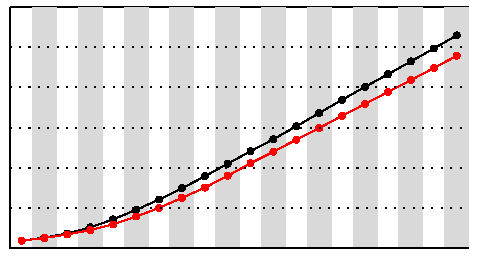
\includegraphics[scale=1.1]{figs/prioraug/uni_data.pdf}};
  \node[rotate=90] at (-4.8,0) {Mean size of data set};
  \node[anchor=east] at (-4.4,2.2) {1200};   \node[anchor=east] at (-4.4,-2.2) {0};
  \node at (0,-2.6) {Algorithm Iteration};
  \node at (-4.1,-2.55) {0};  \node at (4.0,-2.55) {20};
\end{tikzpicture}
\caption{Average data set growth corresponding to the Monte Carlo runs shown in \Fig{uni_sta}. All the data sets grew at around the same rate (represented by the black line) with the exception of the Euler method which grew more slowly due to its poorer performance.}
\label{fig:uni_datasize}
\end{figure}
%-------------------------------------------------------------------------------------------------------------------------------------------




\subsubsection{Results}

The results of running the algorithm with various position reconstruction methods are shown in \Fig{uniplots}. No additional additive noise term was applied in these simulations since it was found that no further improvement could be obtained for this problem.

\Fig{uni_sta} shows the cost trajectory of the standard algorithm as the iterations progress. In crude terms it can be seen that most runs have converged on the ``best" solution by the 14$\tth$ or 15$\tth$ iteration. Moving to the Euler approximation shown in \Fig{uni_eul} it is surprising to see that the algorithm can still solve the learning problem but with generally poorer performance than the standard method. The Heun method produces results comparable to that of the standard method but with arguably slightly faster convergence. Further, the number of runs that fail or incur a high cost in the last 5 iterations is much less than is observed when using the standard method.

Finally, interesting results can be observed with use of the Cubic method. This method achieves the fastest convergence to its final solution with almost all the runs completed by the 11$\tth$ iteration, an improvement over all the other methods. However, the stabilising solution it has found is marginally poorer in terms of cost than the others. This can be put down to overconfidence in the predictive power of the method. 
%
We note that using velocity reconstruction led to variance explosion in the state prediction and numerically unstable results for all methods when applied to this problem and therefore learning was impossible.

%TRY 3rd and 4th ORDER APPROXIMATIONS



%-------------------------------------------------------------------------------------------------------------------------------------------
%\begin{figure}[t!]
%\centering \footnotesize
%\begin{tikzpicture}
%  \node at (0,0) {6 PLOTS, };
%\end{tikzpicture}
%\caption{Sample state trajectory of the stablised unicycle. The top plots show the evolution of the roll $\theta$, pitch $\phi$ and yaw $\psi$ from left to right while the lower plots show the $(x_{\text{c}},y_{\text{c}})$ trajectory followed by the applied wheel torque $u_{\text{w}}$ and turntable torque $u_{\text{t}}$.}
%\label{fig:unitraj}
%\end{figure}
%-------------------------------------------------------------------------------------------------------------------------------------------


\subsubsection{Computational Savings}
As mentioned in the pendulum problem, one of the most appealing aspects of including prior information is in terms of computational saving in the policy optimisation stage of the algorithm. For the unicycle this really is the bottleneck in terms of the speed of the algorithm. During the 20 iterations of the algorithm the data set usually gets up to around 1100 points. The average growth of the data sets for the Monte Carlo runs of the standard algorithm, depicted in \Fig{uni_sta}, are shown by the black line in \Fig{uni_datasize}. The same growth was observed when using the Heun and the Cubic method with a slightly slower growth observed when the Euler method was employed (depicted by the red line), due to slower learning. As expected from the use of a sparse approximation the plots appear to be following a linear growth. Using the Euler or Heun methods leads to reduction of around 40\% in computation while use of state information from $k-2$ leads to around a 30\% reduction. These figures indicate a significant time saving since function evaluations take of the order of one minute for the standard method and therefore around one hour is needed for a single policy optimisation consisting of 60 evaluations.





%-------------------------------------------------------------------------------------------------------------------------------------------
\begin{figure}
\centering \small
\begin{tikzpicture}
  \node at (0,0) {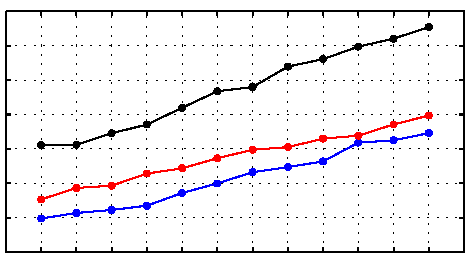
\includegraphics[scale=1.1]{figs/prioraug/uni_timing.pdf}};
  \node[rotate=90] at (-4.7,0) {CPU time (s)};
  \node[anchor=east] at (-4.3,2.2) {90};   \node[anchor=east] at (-4.3,-2.2) {20};
  \node at (0,-2.62) {Training data set size};
  \node at (-3.65,-2.55) {100};  \node at (3.65,-2.55) {1200};
\end{tikzpicture}
\caption{Comparison of CPU time for a single cost function evaluation $J(\bpsi)$ (with derivatives)  for the unicycle with $H = \big\lceil 10/\Dt \big\rceil$ and $\Dt = 0.15\,$s. The black line is for prediction of $\theta$ and $\dot\theta$ with GPs. The blue line is for the case where position states are reconstructed using information back to time $k-1$ and the red line for information back to $k-2$. The x-axis depicts the size of training data set available to the GP.}
\label{fig:unicomps}
\end{figure}
%-------------------------------------------------------------------------------------------------------------------------------------------




\section{Reference Tracking}
\label{sec:reffy}



\subsection{Problem Formulation}
An extension of the regulation problem given by \Eq{Jcost} is now considered. In particular, the problem of forcing a linear combination of the system states $\bC\bx^{\bx}$ to track some reference $\br = \bC^{\br}\bx^{\br}$ where $\bx^{\br} \in \RR^{E_r}$ is the underlying reference state. This will be achieved using a parameterised control policy $\bpi$ which has access to a subset of the full reference state $\bx^{\br}_k[\bi]$ where $\bi$ indicates which elements the policy can use. Mathematically, this problem can be posed as
\begin{align}
& \text{minimise} & J(\bpsi) = \EE_{\btau}\Bigg[ & \sum_{k=0}^{H} c\big(\bC\bx^{\bx}_k - \bC^{\br}\bx^{\br}_k,\bu_k\big) \, \bigg| \, p(\bx^{\bx}_0, \bx^{\br}_0) \Bigg]
\label{eqn:reftrack1} \\
&\text{subject to} & \bx^{\bx}_k &= \bff_{\bx}\big(\bx^{\bx}_{k-1},\bu_{k-1}\big) 
\quad \text{where} \quad \bff_{\bx} \sim p\big(\bff_{\bx}|\cD,\hyp\big) & \label{eqn:reftrack2}\\
\nonumber && \bx^{\br}_k &= \bff_{\br}\big(\bx^{\br}_{k-1}\big) \\
\nonumber && \bu_k &= \bpi\big(\bx^{\bx}_k, \bx^{\br}_k[\bi] \big)
\end{align}
where $\btau := [\bx^{\bx}_0; \bx^{\br}_0; \bu_0 \dots \bx^{\bx}_H]$ is a sampled state-action and reference trajectory. The system dynamics evolve according to the function $\bff_\bx$ while the reference signal is governed by the reference generator $\bff_\br$. We note that $\bff_\br$ may be provided by the user or inferred from data in the same way that we infer the system dynamics. 

In the spirit of \cite{BGW90}, the problem in \Eqs{reftrack1}{reftrack2} can be recast as a regulation problem in terms of an augmented state space and dynamics model. First define the augmented state as $\bx := [\bx^{\bx}; \bx^{\br}]$. Next define the augmented dynamical system
\begin{equation*}
\bx_{k} =
\bff(\bx_{k-1}, \bu_{k-1}) = \bmat{
\bff_{\bx}\big(\bx^{\bx}_{k-1},\bu_{k-1}\big) \\
\bff_{\br}\big(\bx^{\br}_{k-1}\big)
}
\end{equation*}
and the stage-cost $c^{\br}\big(\bx,\bu\big) := c\big([\bC, -\bC^{\br}]\bx,\bu\big)$. The recast problem can now be stated as a regulation problem in terms of the augmented state space
\begin{align}
& \text{minimise} & J(\bpsi) = \EE_{\btau}\Bigg[ & \sum_{k=0}^{H} c^{\br}\big(\bx_k ,\bu_k \big)  \, \bigg| \, p(\bx_0) \Bigg]
 \\
&\text{subject to} & \bx_k &= \bff\big(\bx_{k-1},\bu_{k-1}\big) 
\quad \text{where} \quad \bff \sim p\big(\bff|\cD,\hyp\big) & \\
\nonumber && \bu_k &= \bpi\big( \bx_k[\bj] \big)
\end{align}
where $\bj=[\mathbf{1}; \bi]$ is the new indexing vector. This is in exactly the same form as the original regulation problem posed in \Eqs{learn1}{learn2}. Note that if the moments of the stage-cost $c$ are tractable given a Gaussian input $\bx,\bu \sim \cN$ then so will the moments of $c^{\br}$ since the state has simply undergone a linear transformation and therefore remains Gaussian.



%-------------------------------------------------------------------------------------------------------------------------------------------
\begin{figure}[t]
\centering
\tikzstyle{line} = [draw, -latex]
%
\subfigure[Steps]{
\begin{tikzpicture}
	\footnotesize
	\node at (0,0) {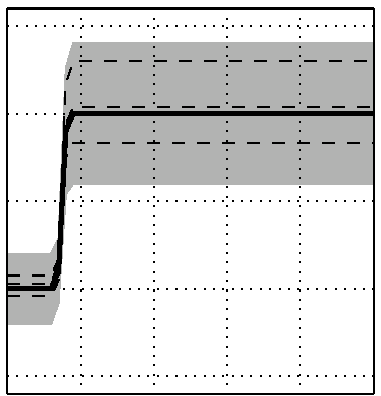
\includegraphics[scale=0.7, clip, trim = .1cm 0cm .1cm 0cm]{figs/prioraug/ref_step.pdf}};
	\node at (0.2,-2.65) {time $(k)$}; \node at (-1.8,1.8) {$r_k$};
	\node at (-2.35,2.1) {1}; \node at (-2.35,0) {0};	\node at (-2.4,-2.1) {-1};
	\node at (-2.1,-2.6) {0};
	\node at (2.05,-2.6) {50};
\end{tikzpicture}
\label{fig:linref1}
}
%
\subfigure[Periodic Waves]{
\begin{tikzpicture}
	\footnotesize
	\node at (0,0) {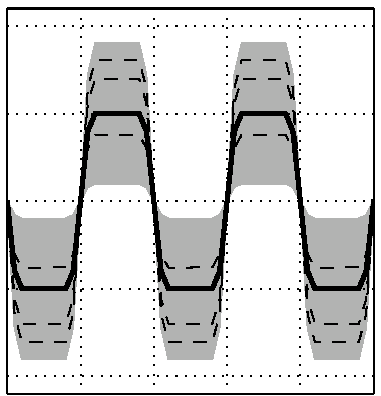
\includegraphics[scale=0.7, clip, trim = .1cm 0cm .1cm 0cm]{figs/prioraug/ref_square.pdf}};
	\node at (0.2,-2.65) {time $(k)$}; \node at (-1.8,1.8) {$r_k$};
	\node at (-2.35,2.1) {1}; \node at (-2.35,0) {0};	\node at (-2.4,-2.1) {-1};
	\node at (-2.1,-2.6) {0};
	\node at (2.05,-2.6) {50};
\end{tikzpicture}
\label{fig:linref2}
}
%
\subfigure[Filtered Noise]{
\begin{tikzpicture}
	\footnotesize
	\node at (0,0) {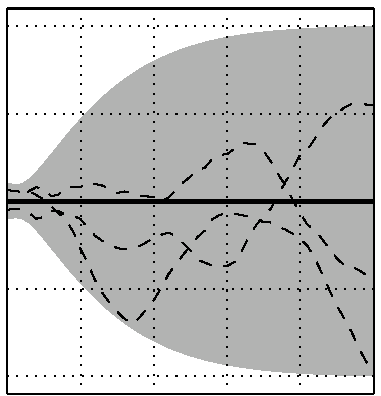
\includegraphics[scale=0.7, clip, trim = .1cm 0cm .1cm 0cm]{figs/prioraug/ref_noise.pdf}};
	\node at (0.2,-2.65) {time $(k)$}; \node at (-1.8,1.8) {$r_k$};
	\node at (-2.35,2.1) {1}; \node at (-2.35,0) {0};	\node at (-2.4,-2.1) {-1};
	\node at (-2.1,-2.6) {0};
	\node at (2.05,-2.6) {50};
\end{tikzpicture}
\label{fig:linref3}
}
%
\caption{Examples of reference signals generated from the linear system $\bx^{\br}_k = \bA^{\br}\bx^{\br}_{k-1} + \bb^{\br}e_{k-1}$ where $r_k = [1,\bO]\bx^{\br}$. Plots (a)-(c) were generated using $\bA^{\br}_1, \bb^{\br}_1$, $\bA^{\br}_2, \bb^{\br}_2$ and $\bA^{\br}_3, \bb^{\br}_3$ respectively. The means are plotted in thick solid lines, samples shown by dashed lines and the $2\sigma$ confidence region shaded in grey.}
\label{fig:linrefs}
\end{figure}
%-------------------------------------------------------------------------------------------------------------------------------------------



\subsection{Preview Horizon}
An important point to make is that the problem given in \Eqs{reftrack1}{reftrack2} can handle the situation in which the control policy is allowed to anticipate the impending change in reference by having access to some \textit{preview horizon} of the reference signal. In other words $\bu_k$ is allowed to be functionally dependent on $\br_{k+i}$ for $i \in \ZZ_{[0,H_{\te{p}}]}$ and a preview horizon of $H_{\te{p}}$ steps. This situation can be encoded by defining the reference state to consist of future values of $\br$ over the preview horizon window $\bx^{\br}_k = [\br_k; \br_{k+1} \dots \br_{k+H_{\te{p}}}]$. Then defining the reference dynamics to consist of
\begin{equation*}
\bx^{\br}_{k+1} = \bff_{\br}\big( \bx^{\br}_{k} \big) = \bmat{
\big[\bO \;\; \bI\big] \bx^{\br}_{k} \\[0.1cm]
\bff_{r}(\br_{k+H_{\te{p}}})
}
\end{equation*}
the problem is back into the form outlined in the previous section. This reference tracking work was originally proposed in \cite{HRM11}.









\subsection{Reference Dynamics}

When considering what kind of reference dynamics model to use it is worth noting that many standard reference signals can be generated using a simple linear system of equations. Some examples are given in \Fig{linrefs}. These were generated using $\bx^{\br}_k = \bA^{\br}\bx^{\br}_{k-1} + \bb ^{\br}e_{k-1}$ where $r_k = [1,\bO]\bx^{\br}$, $\bx^{\br} \sim \cN$ and $e_k \sim \cN(0,1)$. In particular \Fig{linrefs}(a-c) were generated using 
\begin{align*}
\bA_1^{\br} &= \bmat{\bO & \bI \\ 0 & \big[\bO \;\; 1\big]} \in \RR^{10}, \quad
\bA_2^{\br} = \bmat{\bO & \bI \\ -1 & \bO} \in \RR^{10}, \quad
\bA_3^{\br} = \bmat{a & b \\ 0 & a} \in \RR^{2} 
\end{align*}
and $\bb_1^{\br} = \bb_2^{\br} = \bO$, $\bb_3^{\br} = [0;c]$ respectively, along with an appropriate distribution over the start state $\bx^{\br}_0$. The constants $a,b$ and $c$ were chosen such that $\cov[r_k] \rightarrow \big(\tfrac{1}{2}\big)^2$ as $k \rightarrow \infty$ where $|a| <1$ is necessary for a stable generator.



We note that an advantage of the learning framework is that the reference generating system could also be inferred directly from the data, in the same way that standard dynamics are learned. For example, if the reference signals for a system came from a human operator then a Gaussian process model could be trained to imitate the trajectories the operator is producing and used for offline simulation.









\subsection{Example: Cart-pole}



\subsubsection{Setup}
For illustrative purposes, consider the problem of tracking a moving setpoint using the cart-pole set up in \Fig{cartpole}. The equations of motion and constant values for this system can be found in \App{cart}.
The tracking task is to follow a moving $x$, denoted $r$, position with the pole balanced upright. The initial state of the system is at the origin $\bx_0 = \bO$. The stage-cost is in the same form as the unicycle cost in \Eq{unicost} in which $c(\bx) = 1 - \exp\big(-\tfrac{1}{2}d(\bx)^2\big)$ where $d(\bx)^2$ is the squared distance from the setpoint. The distance, in this case can be decomposed as $d(\bx)^2 = d_x^2 + d_z^2$ where
\begin{align*}
d_x &= (x-r) + \sin\theta \\
d_z &= \cos\theta
\end{align*}
The prediction horizon was set to $T = 5\,$s with a discretisation time of $\delta_t = 0.1\,$s leading to $H = 50$ steps. The trials at each iteration of the algorithm were stopped if the pole fell. The Gaussian process model trained to learn the dynamics was initialised with five trial runs in which random inputs were applied. This led to an overall experience of around 1.5$\,$s. Four independent GPs with squared exponential covariance functions were used to learn the dynamics. Finally, the structure of the policy was linear and pushed through the standard saturation block to satisfy the input constraints.

%-------------------------------------------------------------------------------------------------------------------------------------------
\begin{figure}
\centering
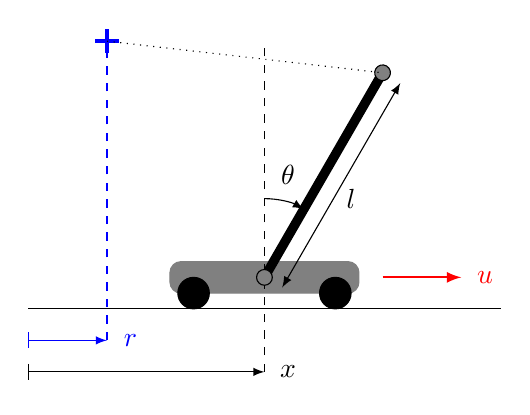
\begin{tikzpicture}[scale=1]
	
	\draw[fill=black!50, black!50, rounded corners] (-1.2,-0.2) rectangle (1.2,0.2); % body
	\draw[fill=black] (0.9,-0.2) circle (.2cm); \draw[fill=black] (-0.9,-0.2) circle (.2cm); % wheels
	\draw[black, line width = 1.2mm, rotate=-30] (0,0) -- (0,3); % pole
	
	\draw[fill=gray, rotate=-30] (0,3) circle (1mm);
	\draw[dashed] (0,-1.2) -- (0,3);
	\draw[dashed, blue] (-2,-0.8) -- (-2,3);
	\draw[rotate=90, -latex] (1,0) arc (0:-30:1cm);
	\draw[fill=gray] (0,0) circle (1mm);
	
	\node[] at (0.3,1.3) {$\theta$};
	\node[] at (1.1,1.0) {$l$};
	
	
	\draw[xshift=0.3cm,rotate=-30,-latex] (0,0) -- (0,2.85); \draw[xshift=0.3cm,rotate=-30,-latex] (0,0) -- (0,-0.15);
	
	\draw[very thick, blue] (-2,2.85) -- (-2,3.15); \draw[very thick, blue] (-1.85,3) -- (-2.15,3);
	\draw[dotted] (-2,3) -- (1.5,2.5981);
	
	\draw[] (-3,-0.4) -- (3,-0.4);
	
	\node[] at (-1.7,-0.8) {\color{blue} $r$};
	\draw[blue] (-3, -0.7) -- (-3,-0.9);
	\draw[blue,-latex] (-3, -0.8) -- (-2,-0.8);
	
	\node[] at (0.3,-1.2) {$x$};
	\draw[] (-3, -1.1) -- (-3,-1.3);
	\draw[-latex] (-3, -1.2) -- (0,-1.2);
	
	\node[] at (2.8,0) {\color{red}$u$};
	\draw[-latex, red, thick] (1.5, 0) -- (2.5,0);

	
\end{tikzpicture}
\caption{Cart-pole setup with position $x$,  pole angle $\theta$, pole length $l$, action force $u$ and lateral location of the setpoint $r$. The setpoint is shown by the blue cross and the Euclidean distance from the tip of the pole to the setpoint is shown by the dotted line. }
\label{fig:cartpole}
\end{figure}
%-------------------------------------------------------------------------------------------------------------------------------------------









%-------------------------------------------------------------------------------------------------------------------------------------------
\begin{figure}
\centering \footnotesize
\subfigure[No preview horizon]{ % Hp = 1
\begin{tikzpicture}
  \node at (0,0) {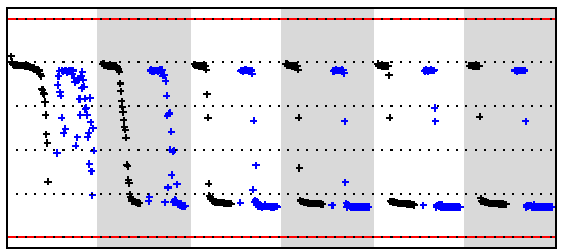
\includegraphics[scale = 0.75]{figs/prioraug/cartcost1.pdf}};
  \node[rotate=90] at (-3.75,0) {Cost};
  \node at (-3.7,1.35) {1}; \node at (-3.7,-1.4) {0};
\end{tikzpicture}
\label{fig:cart01}
}
\subfigure[Preview horizon $T_{\te{p}} = 0.1\,$s]{ % Hp = 2
\begin{tikzpicture}
  \node at (0,0) {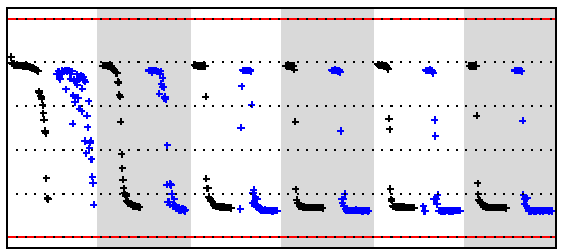
\includegraphics[scale = 0.75]{figs/prioraug/cartcost2.pdf}};
  \node[rotate=90] at (-3.75,0) {Cost};
  \node at (-3.7,1.35) {1}; \node at (-3.7,-1.4) {0};
\end{tikzpicture}
\label{fig:cart02}
}
\subfigure[Preview horizon $T_{\te{p}} = 0.3\,$s]{ % Hp = 4
\begin{tikzpicture}
  \node at (0,0) {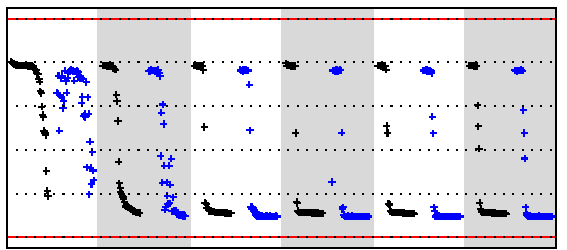
\includegraphics[scale = 0.75]{figs/prioraug/cartcost3.pdf}};
  \node[rotate=90] at (-3.75,0) {Cost};
  \node at (-3.7,1.35) {1}; \node at (-3.7,-1.4) {0};
\end{tikzpicture}
\label{fig:cart03}
} 
\subfigure[Preview horizon $T_{\te{p}} = 1.0\,$s]{ % Hp = 10
\begin{tikzpicture}
  \node at (0,0) {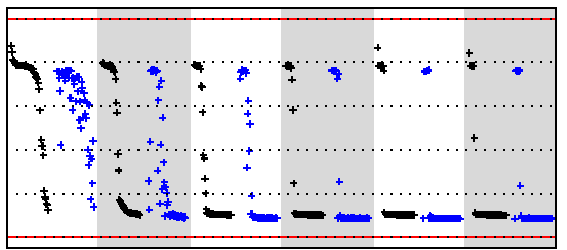
\includegraphics[scale = 0.75]{figs/prioraug/cartcost4.pdf}};
  \node[rotate=90] at (-3.75,0) {Cost};
  \node at (-3.7,1.35) {1}; \node at (-3.7,-1.4) {0};
\end{tikzpicture}
\label{fig:cart04}
}
\caption{Cost incurred by the current policy after a given iteration of the algorithm. The policy has access to different preview horizons $T_{\te{p}}$ of the reference. Black crosses show the actual cost incurred while the blue shows the mean predicted cost. }
\label{fig:cartcosts}
\end{figure}
%-------------------------------------------------------------------------------------------------------------------------------------------


%-------------------------------------------------------------------------------------------------------------------------------------------
\begin{figure}
\centering \footnotesize
\subfigure[No preview horizon]{ % Hp = 1
\begin{tikzpicture}
  \node at (0,3) {};
  \node at (0,0) {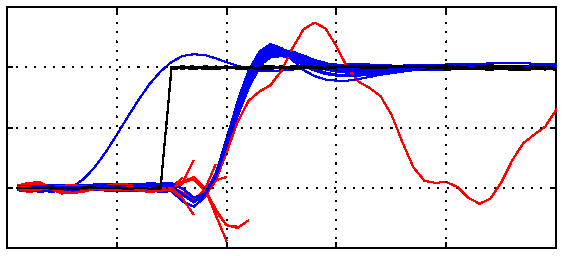
\includegraphics[scale = 0.75]{figs/prioraug/cart_step1.pdf}};
  \node at (-2.75,1.1) {$x\,$(m)};
  \node at (0,-2.1) {time$\,$(s)};
  \node at (-3.65,-0.75) {0};  \node at (-3.65,0.75) {1};
  \node at (-3.5,-1.8) {0};  \node at (-2.1,-1.8) {1};  \node at (-0.7,-1.8) {2};
  \node at (0.7,-1.8) {3};  \node at (2.1,-1.8) {4};  \node at (3.5,-1.8) {5};
\end{tikzpicture}
}
\subfigure[Preview horizon $T_{\te{p}} = 0.1\,$s]{ % Hp = 2
\begin{tikzpicture}
  \node at (0,0) {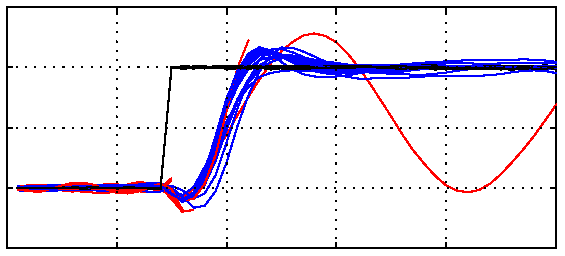
\includegraphics[scale = 0.75]{figs/prioraug/cart_step2.pdf}};
  \node at (-2.75,1.1) {$x\,$(m)};
  \node at (0,-2.1) {time$\,$(s)};
  \node at (-3.65,-0.75) {0};  \node at (-3.65,0.75) {1};
  \node at (-3.5,-1.8) {0};  \node at (-2.1,-1.8) {1};  \node at (-0.7,-1.8) {2};
  \node at (0.7,-1.8) {3};  \node at (2.1,-1.8) {4};  \node at (3.5,-1.8) {5};
\end{tikzpicture}
}
\subfigure[Preview horizon $T_{\te{p}} = 0.3\,$s]{ % Hp = 4
\begin{tikzpicture}
  \node at (0,0) {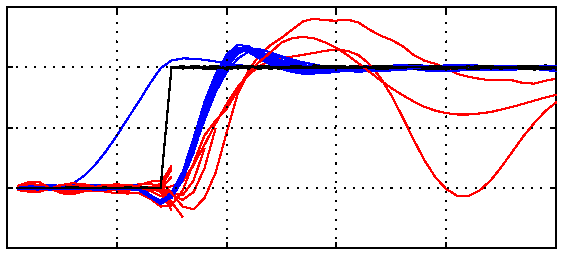
\includegraphics[scale = 0.75]{figs/prioraug/cart_step3.pdf}};
  \node at (-2.75,1.1) {$x\,$(m)};
  \node at (0,-2.1) {time$\,$(s)};
  \node at (-3.65,-0.75) {0};  \node at (-3.65,0.75) {1};
  \node at (-3.5,-1.8) {0};  \node at (-2.1,-1.8) {1};  \node at (-0.7,-1.8) {2};
  \node at (0.7,-1.8) {3};  \node at (2.1,-1.8) {4};  \node at (3.5,-1.8) {5};
\end{tikzpicture}
}
\subfigure[Preview horizon $T_{\te{p}} = 1.0\,$s]{ % Hp = 10
\begin{tikzpicture}
  \node at (0,0) {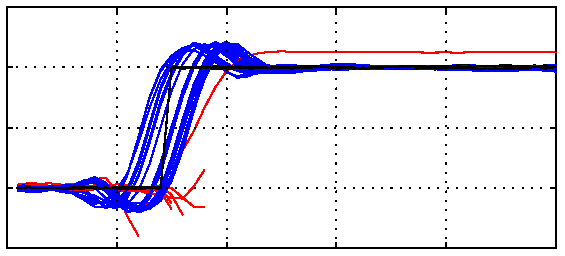
\includegraphics[scale = 0.75]{figs/prioraug/cart_step4.pdf}};
  \node at (-2.75,1.1) {$x\,$(m)};
  \node at (0,-2.1) {time$\,$(s)};
  \node at (-3.65,-0.75) {0};  \node at (-3.65,0.75) {1};
  \node at (-3.5,-1.8) {0};  \node at (-2.1,-1.8) {1};  \node at (-0.7,-1.8) {2};
  \node at (0.7,-1.8) {3};  \node at (2.1,-1.8) {4};  \node at (3.5,-1.8) {5};
\end{tikzpicture}
}
\caption{Responses of the cart-pole system corresponding to the costs depicted in \Fig{cartcosts} at the sixth iteration. The policy preview horizon $T_{\te{p}}$ was altered between these four sets of runs. The runs show the step responses of 50 runs after the 10th iteration of the algorithm. Red lines show runs in which the pole falls over or can balance but have not learned to track yet.}
\label{fig:cartplots}
\end{figure}
%-------------------------------------------------------------------------------------------------------------------------------------------



\subsubsection{Results}
The first task the cart-pole system was tasked with was to learn a policy to track a unit step change in position $x$ occurring at 1.5$\,$s. The available preview horizon $T_{\te{p}}$ was varied from $0$ to $1\,$s to investigate the effect of allowing the policy to anticipate the change in setpoint. The predicted and actual costs of 50 Monte Carlo runs over 6 algorithm iterations are shown in \Fig{cartcosts}. It is clear that many runs reach their solution after only two iterations while most finish learning after just three. Further note the decrease in cost of the best solution as the preview horizon is increased. This demonstrates that, as we would expect, being able to anticipate the change is beneficial. Note that there is a failure mode that a significant number of the runs end up in. In this mode the pole is balanced at the origin until the change in setpoint then the policy allows it to fall over! There are also a couple of runs that can keep the pole balanced but have not yet learned to track the setpoint.





The actual solutions to which the algorithm converged are given in \Fig{cartplots}. The blue lines correspond to runs that kept the pole upright while the red lines correspond to the failure mode and runs that did not keep the pole balanced. Note that as the preview horizon is increased the benefit of being able to anticipate the change in setpoint is clear. An interesting artefact from the $T_{\te{p}} = 1.0\,$s runs is that there are two optimal solutions, one in which the cartpole moves so that it is in position at the new setpoint when it changes and one in which it is ready to move as the setpoint changes.
%
Another interesting result from using no preview horizon or $T_{\te{p}} = 0.3\,$s can be observed in \Fig{cart01} and (c). In these cases the policy has chosen to ignore the setpoint reference signal and simply regulate to the $x=1\,$m position. This behaviour results from only considering a single setpoint change rather than a distribution of possible changes.



%-------------------------------------------------------------------------------------------------------------------------------------------
\begin{figure}
\centering \footnotesize
\subfigure[No preview horizon]{ % Hp = 1
\begin{tikzpicture}
  \node at (0,0) {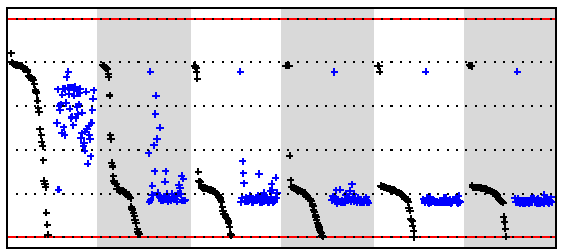
\includegraphics[scale = 0.75]{figs/prioraug/cartcost5.pdf}};
  \node[rotate=90] at (-3.75,0) {Cost};
  \node at (-3.7,1.35) {1}; \node at (-3.7,-1.4) {0};
\end{tikzpicture}
\label{fig:cart05}
}
\subfigure[Preview horizon $T_{\te{p}} = 0.1\,$s]{ % Hp = 2
\begin{tikzpicture}
  \node at (0,0) {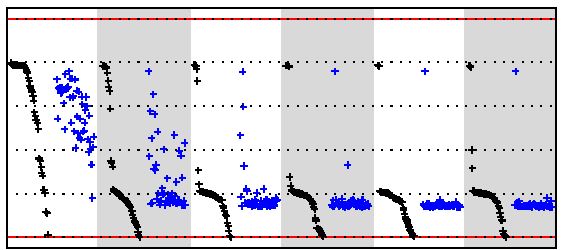
\includegraphics[scale = 0.75]{figs/prioraug/cartcost6.pdf}};
  \node[rotate=90] at (-3.75,0) {Cost};
  \node at (-3.7,1.35) {1}; \node at (-3.7,-1.4) {0};
\end{tikzpicture}
\label{fig:cart06}
}
\subfigure[Preview horizon $T_{\te{p}} = 0.3\,$s]{ % Hp = 4
\begin{tikzpicture}
  \node at (0,0) {\includegraphics[scale = 0.75]{figs/prioraug/cartcost7.pdf}};
  \node[rotate=90] at (-3.75,0) {Cost};
  \node at (-3.7,1.35) {1}; \node at (-3.7,-1.4) {0};
\end{tikzpicture}
\label{fig:cart07}
} 
\subfigure[Preview horizon $T_{\te{p}} = 1.0\,$s]{ % Hp = 10
\begin{tikzpicture}
  \node at (0,0) {\includegraphics[scale = 0.75]{figs/prioraug/cartcost8.pdf}};
  \node[rotate=90] at (-3.75,0) {Cost};
  \node at (-3.7,1.35) {1}; \node at (-3.7,-1.4) {0};
\end{tikzpicture}
\label{fig:cart08}
}
\caption{Cost incurred by the algorithm by applying the current best policy after a given iteration (given by the x-axis). Black crosses show the actual cost incurred while the blue shows the predicted cost. }
\label{fig:cartcosts2}
\end{figure}
%-------------------------------------------------------------------------------------------------------------------------------------------


We can of course optimise over a distribution over trajectories as shown in \Fig{linrefs}. The next set of simulations was trained using a step change model that changed at the same time as before but the new setpoint was sampled from the distribution $\cN(0,1)$. The results of learning a control policy to achieve this task are shown in \Fig{cartcosts2}. The first thing to note is that the resulting spread in the actual costs as learning proceeds is not emulated in the predicted costs because the predictions are of the average cost that will be incurred. Bearing this in mind, the predictions match up well with the actual performance. We can again see a significant improvement in performance as the preview horizon is increased.

The most notable feature of these results is that we no longer fall into the same failure models that we did when we considered only a deterministic change in setpoint. With the exception of two, all these runs learned how to track a given setpoint. The only runs that failed were the ones that had to track setpoint changes greater than around 2$\,$m. This makes sense since this is the 2$\sigma$ point for the setpoint distribution.




%-------------------------------------------------------------------------------------------------------------------------------------------
\begin{figure}
\centering \footnotesize
\subfigure[Access only to the reference position]{ % Hp = 1
\begin{tikzpicture}
  \node at (0,0) {\includegraphics[scale = 0.75]{figs/prioraug/cartcost9.pdf}};
  \node[rotate=90] at (-3.75,0) {Cost};
  \node at (-3.7,1.35) {1}; \node at (-3.7,-1.4) {0};
\end{tikzpicture}
\label{fig:cart09}
}
\subfigure[Access to the full reference state.]{ % Hp = 2
\begin{tikzpicture}
  \node at (0,0) {\includegraphics[scale = 0.75]{figs/prioraug/cartcost10.pdf}};
  \node[rotate=90] at (-3.75,0) {Cost};
  \node at (-3.7,1.35) {1}; \node at (-3.7,-1.4) {0};
\end{tikzpicture}
\label{fig:cart10}
}
\caption{Cost incurred by the algorithm by applying the current best policy after a given iteration (given by the x-axis). Black crosses show the actual cost incurred while the blue shows the predicted cost. }
\label{fig:cartcosts3}
\end{figure}
%-------------------------------------------------------------------------------------------------------------------------------------------


The final set of simulations we carried out was to track references generated by the second order filter depicted in \Fig{linref3}. In particular, the reference system we considered was given by
\begin{equation*}
\bx^{\br}_{k+1} = \bmat{0.92 & 2.22 \\ 0 & 0.92}\bx^{\br}_{k} + \bmat{0 \\ 0.1}e_k
\end{equation*}
with $\bx^{\br}_0 = \bO$. In the limit of $k\rightarrow \infty$ the standard deviation of the position term saturates to 0.5$\,$m. We first gave the policy access only to the positional term and the results are shown in \Fig{cart09}. Then we gave the policy access to the full reference state and obtained the results in \Fig{cart10}. These results clearly show that the learning procedure has exploited the additional information to obtain much improved tracking performance.






%-------------------------------------------------------------------------------------------------------------------------------------------
\begin{figure}
\centering \footnotesize
\subfigure[Spinning on the spot]{ % Hp = 1
\begin{tikzpicture}
  \node at (-5.3,0) {\includegraphics[scale = 0.7]{figs/prioraug/uni_spin1_1.pdf}};
  \node at (0,0) {\includegraphics[scale = 0.7]{figs/prioraug/uni_spin1_2.pdf}};
  \node at (-10.6,0) {\includegraphics[scale = 0.7]{figs/prioraug/uni_spin1_3.pdf}};
  
  % y coords
  \node at (-7.7,2) {$x_\te{c}$}; \node at (-7.7,1.3) {1}; \node at (-7.7,0) {0}; \node at (-7.7,-1.3) {-1};
  \node at (-2.4,2) {$y_\te{c}$}; \node at (-2.4,1.3) {1}; \node at (-2.4,0) {0}; \node at (-2.4,-1.3) {-1};
  \node at (-13,2) {$y$}; \node at (-13,1.3) {1}; \node at (-13,0) {0}; \node at (-13,-1.3) {-1};
  
  % x coords
  \node at (-7.4,-2.55) {0}; \node at (-5.3,-2.6) {time (s)}; \node at (-3.2,-2.55) {20};
  \node at (-2.1,-2.55) {0}; \node at (0,-2.6) {time (s)}; \node at (2.1,-2.55) {20};
  \node at (-8.6,-2.55) {$x$}; \node at (-11.9,-2.55) {-1}; \node at (-10.6,-2.55) {0}; \node at (-9.3,-2.55) {1};
\end{tikzpicture}
\label{fig:uni01}
}
\subfigure[Spin whilst moving slowly round the circle]{ % Hp = 1
\begin{tikzpicture}
  \node at (-5.3,0) {\includegraphics[scale = 0.7]{figs/prioraug/uni_spin2_1.pdf}};
  \node at (0,0) {\includegraphics[scale = 0.7]{figs/prioraug/uni_spin2_2.pdf}};
  \node at (-10.6,0) {\includegraphics[scale = 0.7]{figs/prioraug/uni_spin2_3.pdf}};
  
  % y coords
  \node at (-7.7,2) {$x_\te{c}$}; \node at (-7.7,1.3) {1}; \node at (-7.7,0) {0}; \node at (-7.7,-1.3) {-1};
  \node at (-2.4,2) {$y_\te{c}$}; \node at (-2.4,1.3) {1}; \node at (-2.4,0) {0}; \node at (-2.4,-1.3) {-1};
  \node at (-13,2) {$y$}; \node at (-13,1.3) {1}; \node at (-13,0) {0}; \node at (-13,-1.3) {-1};
  
  % x coords
  \node at (-7.4,-2.55) {0}; \node at (-5.3,-2.6) {time (s)}; \node at (-3.2,-2.55) {20};
  \node at (-2.1,-2.55) {0}; \node at (0,-2.6) {time (s)}; \node at (2.1,-2.55) {20};
  \node at (-8.6,-2.55) {$x$}; \node at (-11.9,-2.55) {-1}; \node at (-10.6,-2.55) {0}; \node at (-9.3,-2.55) {1};
\end{tikzpicture}
\label{fig:uni02}
}
\subfigure[Spin whilst moving rapidly round the circle]{ % Hp = 2
\begin{tikzpicture}
  \node at (-5.3,0) {\includegraphics[scale = 0.7]{figs/prioraug/uni_spin3_1.pdf}};
  \node at (0,0) {\includegraphics[scale = 0.7]{figs/prioraug/uni_spin3_2.pdf}};
  \node at (-10.6,0) {\includegraphics[scale = 0.7]{figs/prioraug/uni_spin3_3.pdf}};
  
  % y coords
  \node at (-7.7,2) {$x_\te{c}$}; \node at (-7.7,1.3) {1}; \node at (-7.7,0) {0}; \node at (-7.7,-1.3) {-1};
  \node at (-2.4,2) {$y_\te{c}$}; \node at (-2.4,1.3) {1}; \node at (-2.4,0) {0}; \node at (-2.4,-1.3) {-1};
  \node at (-13,2) {$y$}; \node at (-13,1.3) {1}; \node at (-13,0) {0}; \node at (-13,-1.3) {-1};
  
  % x coords
  \node at (-7.4,-2.55) {0}; \node at (-5.3,-2.6) {time (s)}; \node at (-3.2,-2.55) {20};
  \node at (-2.1,-2.55) {0}; \node at (0,-2.6) {time (s)}; \node at (2.1,-2.55) {20};
  \node at (-8.6,-2.55) {$x$}; \node at (-11.9,-2.55) {-1}; \node at (-10.6,-2.55) {0}; \node at (-9.3,-2.55) {1};
\end{tikzpicture}
\label{fig:uni03}
}
\caption{Plots showing the movement of the base of the balanced unicycle as it tracks a spinning setpoint defined in the body-fixed coordinate system $(x_\te{c},y_\te{c})$. The left hand plots show the actual spatial trajectory of the base of the unicycle in blue whilst the red line shows the trajectory of the front of the wheel in order to demonstrate the spinning motion. The other plots show the reference in black and the relevant state of the unicycle in blue.}
\label{fig:uniorbits}
\end{figure}
%-------------------------------------------------------------------------------------------------------------------------------------------





\subsection{Example: Unicycle}
%\subsubsection{Reference Signal}
We now turn our attention back to the unicycle problem of \Sec{unicycle}. We were unsuccessful in getting the unicycle to track specific references in an absolute coordinate system $(x,y)$ however we did succeed in tracking references defined in the body-fixed coordinate system $(x_\te{c},y_\te{c})$ shown in \Fig{unicycle}. Our reasoning for this is that tracking trajectories in the body-fixed coordinate system could be achieved through an infinite number of possible trajectories in an absolute frame of reference. This is because this coordinate system is invariant to rotations around the global origin. Therefore tracking in body-fixed coordinates is less constraining and less challenging than tracking an equivalent fixed trajectory in an absolute frame. This point will be illustrated more clearly with an example.

We tasked the unicycle to stay on the unit circle in the absolute coordinate system $(x,y)$. In order to do this using absolute coordinates we had to define a reference state space system
\begin{equation*}
\bmat{x^\te{r}_k \\ y^\te{r}_k} = \bmat{ \cos\big(\omega_{\te{o}} \Dt\big) & \sin\big(\omega_{\te{o}} \Dt\big) \\ -\sin\big(\omega_{\te{o}} \Dt\big) & \cos\big(\omega_{\te{o}} \Dt\big) }
\bmat{x^\te{r}_{k-1} \\ y^\te{r}_{k-1}}
\end{equation*}
where $\omega_{\te{o}} = 2\pi/T_{\te{o}}$ with orbital period $T_{\te{o}}$ and we set the initial state $(x^\te{r}_0, y^\te{r}_0)=(0,1)$. The algorithm failed to learn this task for multiple values of $T_{\te{o}}$. It would either balance at the origin or follow an orbital trajectory of random radius, which are local minima of the problem. Even when we set $T_{\te{o}}$ to the value of one of these random orbits the algorithm still failed. However, the problem could be posed in a general way using the body-fixed coordinates $(x_{\te{c}},y_\te{c})$ and simply defining a ``setpoint" of $(x^\te{r}_\te{c},y^\te{r}_\te{c}) = (0,1)$. This ``setpoint'' defines all locations of the unicycle for which the origin is 1$\,$m from its right hand side. Under this setup the algorithm could learn this task slightly quicker than the task of balancing.






After this investigation we defined a more exotic set of trajectories using the reference state space system in body-fixed coordinates given by
\begin{equation*}
\bmat{x^\te{r}_{\te{c},k} \\ y^\te{r}_{\te{c},k}} = \bmat{ \cos\big(\omega_{\te{o}} \Dt\big) & \sin\big(\omega_{\te{o}} \Dt\big) \\ -\sin\big(\omega_{\te{o}} \Dt\big) & \cos\big(\omega_{\te{o}} \Dt\big) }
\bmat{x^\te{r}_{\te{c},k-1} \\ y^r_{\te{c},k-1}}
\end{equation*}
If we now set $(x^\te{r}_{\te{c},0},y^\te{r}_{\te{c},0}) = (0,1)$, this tasks the unicycle to stay on the unit circle but to spin around with a period of $T_{\te{o}}$. Three of the solutions the algorithm learned for $T_\te{o} = 5\,$s are shown in \Fig{uniorbits}. These plots clearly show the variety of solutions available to achieve the same task. The policy guiding the unicycle in \Fig{uni01} simply spins it on the spot, whereas the policies shown in (b) and (c) also travel around the unit circle, at varying speeds. We note that very few of the learned control policies could keep tracking beyond 20$\,$s. This issue highlights one of the problems with only training on a relatively short prediction horizon, in this case 10$\,$s. We did not attempt greater prediction horizons because of the increased computation time required to do this.


Finally, through careful selection of reference generator systems we can train the unicycle to track a figure-of-eight trajectory. For example, this can be achieved using the following state space system
\begin{align*}
\bx^\br_+ &= \bmat{ 
\cos\big(2\omega_{\te{o}} \Dt\big) & \sin\big(2\omega_{\te{o}} \Dt\big) & 0 & 0 \\ 
-\sin\big(2\omega_{\te{o}} \Dt\big) & \cos\big(2\omega_{\te{o}} \Dt\big) & 0 & 0 \\
0 & 0 & \cos\big(\omega_{\te{o}} \Dt\big) & \sin\big(\omega_{\te{o}} \Dt\big) \\
0 & 0 & -\sin\big(\omega_{\te{o}} \Dt\big) & \cos\big(\omega_{\te{o}} \Dt\big)}
\bx^\br \\
\bmat{x^\te{r}_{\te{c},k} \\ y^\te{r}_{\te{c},k}} &= \bmat{1 & 0 & 0 & 0 \\ 0 & 0 & 0 & 1} \bx^\br
\end{align*}
with initial reference state $\bx^\br_0 = [0, 1, 0, 1]\T$. With this setup $x^\te{r}_{\te{c}}$ varies as a sine wave while $y^\te{r}_{\te{c}}$ varies as a cosine wave with twice the period. This was clearly a very difficult problem since we were only able to find one training run, from many attempts, that actually managed to learn a policy which achieved the task. The policy learned after 20 iterations of the algorithm was then run for 30$\,$s and the resulting trajectory is shown in \Fig{uniFOE}. Again, we can see the rotational invariance property of the body-fixed coordinate system as the figure-of-eight is not fixed in absolute coordinates. 




%-------------------------------------------------------------------------------------------------------------------------------------------
\begin{figure}
\centering \footnotesize
\begin{tikzpicture}
  \node at (-5.3,0) {\includegraphics[scale = 0.7]{figs/prioraug/uni_foe_1.pdf}};
  \node at (0,0) {\includegraphics[scale = 0.7]{figs/prioraug/uni_foe_2.pdf}};
  \node at (-10.6,0) {\includegraphics[scale = 0.7]{figs/prioraug/uni_foe_3.pdf}};
  
  % y coords
  \node at (-7.7,2) {$x_\te{c}$}; \node at (-7.7,1.15) {1}; \node at (-7.7,0) {0}; \node at (-7.7,-1.15) {-1};
  \node at (-2.4,2) {$y_\te{c}$}; \node at (-2.4,1.15) {1}; \node at (-2.4,0) {0}; \node at (-2.4,-1.15) {-1};
  \node at (-13,2) {$y$}; \node at (-13,1.15) {1}; \node at (-13,0) {0}; \node at (-13,-1.15) {-1};
  
  % x coords
  \node at (-7.4,-2.55) {0}; \node at (-5.3,-2.6) {time (s)}; \node at (-3.2,-2.55) {30};
  \node at (-2.1,-2.55) {0}; \node at (0,-2.6) {time (s)}; \node at (2.1,-2.55) {30};
  \node at (-8.6,-2.55) {$x$}; \node at (-11.75,-2.55) {-1}; \node at (-10.6,-2.55) {0}; \node at (-9.45,-2.55) {1};
\end{tikzpicture}
\caption{Plots showing the movement of the base of the balanced unicycle as it tracks a figure-of-eight in the body-fixed coordinate system $(x_\te{c},y_\te{c})$. The left hand plots show the actual spatial trajectory of the base of the unicycle in red and the unit circle in black. The other plots show the reference trajectory in black and the relevant state of the unicycle in blue.}
\label{fig:uniFOE}
\end{figure}
%-------------------------------------------------------------------------------------------------------------------------------------------






%In this case the unicycle is no longer be asked to regulate to the origin but to track a moving position on the ground. A bit of work must be done first in order to set this problem up correctly. We shall consider orbits in the global coordinate system $(x,y)$ where $x$ lies along $\bi$ and $y$ lies along $\bj$ from \Fig{unicycle}. First, consider the discrete-time state-space equations describing a circular orbit
%\begin{equation*}
%\bmat{x^r_k \\ y^r_k} = \bmat{ \cos\big(\omega_{\te{o}} \Dt\big) & \sin\big(\omega_{\te{o}} \Dt\big) \\ -\sin\big(\omega_{\te{o}} \Dt\big) & \cos\big(\omega_{\te{o}} \Dt\big) }
%\bmat{x^r_{k-1} \\ y^r_{k-1}}
%\end{equation*}
%where $\omega_{\te{o}} = 2\pi/T_{\te{o}}$ and $T_{\te{o}}$ is the period of the orbit in seconds. The radius of the orbit will depend on the initial conditions $x^r_0$ and $y^r_0$. The problem comes in the fact that the unicycle needs to work in a body-centred coordinate system but currently the reference is in an absolute frame. Therefore the following transformation needs to be done before this reference can be passed to the policy
%\begin{equation*}
%\bmat{x^r_{\te{c}k} \\ y^r_{\te{c}k}} = \bmat{ \cos\psi_k & \sin\psi_k \\ -\sin\psi_k & \cos\psi_k }
%\bmat{x^r_{k} \\ y^r_{k}}
%\end{equation*}
%However, this is a nontrivial task since $\psi$, $x^r_{k}$ and $y^r$ will be jointly Gaussian distributed. In this case we can use the framework provided by augmented dynamics to find a solution. Define the intermediate variables $\ba = [\cos\psi, \sin\psi]\T$, $\bb = [x^r\cos\psi, x^r\sin\psi, y^r\cos\psi, y^r\sin\psi]\T$. Now since we can perform moment matching for linear relationships, trigonometric functions and products of jointly Gaussian variables we can find the distribution of $[x^r_{\te{c}k}, y^r_{\te{c}k}]\T$ given the joint distribution over $[\psi, x^r_{k}, y^r_{k}]\T$. This completes the problem setup.



%The algorithm was run with same parameters as before and for 20 iterations and a prediction horizon of 10$\,$s. The task was to learn a policy to track a circular orbit of of varying periods and 1$\,$m radius. 
%
%This was evidently a difficult task since none of the runs actually managed to track the given target at the correct velocity. However, some interesting insight can be gained. The runs that stayed balanced over the whole time tended to settle into an orbit of varying radius but with period always around 6 to 8$\,$s. Even when the reference period was set in this range the tracking task still failed. 



%We concluded that the reason for the failure of this set of experiments is intrinsic to the unicycle dynamics themselves, which render the problem of position tracking almost impossible. Our reasoning is as follows. It was possible to train the unicycle to orbit around the unit circle by defining the body centred setpoint $(x^r_{\te{c}},y^r_{\te{c}}) = (0,1)$ and tasking the unicycle to ``regulate" to this coordinate. It is clear that this defines every point on the unit circle from \Fig{unicycle2}. The only difference between this task and the reference tracking setup is that we were not asking the unicycle to regulate to a specific moving spatial location.






\section{Summary}
Prior knowledge about a dynamical system often comes in the form of known, or approximate, relationships between subsets of the state variables. We have outlined a method for incorporating this prior knowledge into the general framework of probabilistic learning control outlined in the previous chapter. To achieve this we view the system state as evolving according to multiple dynamics models, or sub-dynamics. The key contribution was then in how to propagate the uncertainty in the predictions, which employed the use of a slightly more restrictive assumption of joint Gaussianity than the assumptions made in the previous chapter.

This method found its most obvious use in encoding position-velocity relationships between state variables and in the modelling of higher order Markov systems. However, we demonstrated that it can also be used to tackle problems of reference tracking in which the system is tasked to regulate to a moving setpoint. In addition to this we can allow the policy to have access to a preview horizon of the reference state and therefore allow the algorithm to learn how best to anticipate a change of setpoint.


We were also interested in the question of how the incorporation of such information would affect the learning speed of the algorithm, both computationally and convergence to a good policy, and the propensity for finding good (or bad) local minima in a given problem. This was examined for the pendulum swing-up and unicycle balancing tasks where we included various approximate models for the position-velocity relationships. As expected, we found that a crude model led to poorer results. However, we found that more elaborate models did not necessarily lead to better solutions. We also noticed that although sometimes the propensity for finding poor locally optimal solutions was decreased in many cases, it was amplified in others, in particular when reconstructing velocity from predictions of the position!

Finally, we demonstrated the capability of the framework to learn reference tracking policies on a simulation of a cart and pole. The policy was able to exploit any preview horizon we gave it to help it anticipate the change. We further noted that learning to track a distribution of possible reference signals led to improved learning performance in terms of avoiding poor local minima. Reference tracking was also shown to work on the unicycle when the reference signal was defined in the body-fixed coordinate system rather than absolute coordinates.